%% LyX 2.3.2 created this file.  For more info, see http://www.lyx.org/.
%% Do not edit unless you really know what you are doing.
\documentclass{article}
\usepackage[utf8]{inputenc}
\usepackage{geometry}
\geometry{verbose,tmargin=2.5cm,bmargin=2cm,lmargin=2cm,rmargin=2cm}
\usepackage{color}
\usepackage{array}
\usepackage{verbatim}
\usepackage{float}
\usepackage{units}
\usepackage{mathtools}
\usepackage{amsmath}
\usepackage{graphicx}

\makeatletter

%%%%%%%%%%%%%%%%%%%%%%%%%%%%%% LyX specific LaTeX commands.
\newcommand{\noun}[1]{\textsc{#1}}
%% Because html converters don't know tabularnewline
\providecommand{\tabularnewline}{\\}

%%%%%%%%%%%%%%%%%%%%%%%%%%%%%% Textclass specific LaTeX commands.
\newcommand{\lyxaddress}[1]{
	\par {\raggedright #1
	\vspace{1.4em}
	\noindent\par}
}

%%%%%%%%%%%%%%%%%%%%%%%%%%%%%% User specified LaTeX commands.
\usepackage{xr}
\externaldocument{Paper_req-550_V0.4}
\usepackage{lineno}
\usepackage{xcolor}
\usepackage{tikz}
\usetikzlibrary{arrows}

\newcommand{\bs}[1]{\boldsymbol{#1}}
\newcommand{\add}[1]{\textcolor{red}{#1}}
\newcommand{\oran}{\mathrm{o}}
\newcommand{\g}{\mathrm{g}}
\newcommand{\X}{\mathrm{X}}
\newcommand{\Y}{\mathrm{Y}}
\newcommand{\PP}{\mathrm{P}}
\newcommand{\EE}{\mathrm{E}}
\newcommand{\HH}{\mathrm{H}}
\newcommand{\A}{\mathrm{A}}
\newcommand{\I}{\mathrm{I}}
\newcommand{\M}{\mathrm{M}}

\newcommand{\sh}{\mathrm{sh}}
\newcommand{\nullm}{\mathrm{null}}
\newcommand{\intv}{\mathrm{intv}}
\newcommand{\family}{\mathrm{visit}}
\newcommand{\care}{\mathrm{care}}
\newcommand{\Exp}{\mathrm{exp}}
\newcommand{\onset}{\mathrm{onset}}

\makeatother

\begin{document}
\title{Supplementary Methods and Results\\Empowering the crowd: Feasible
strategies \\ to minimize the spread of COVID-19 \\ in informal
settlements}
\author{Alberto Pascual-García$^{(1,*)}$, Jordan Klein$^{(2)}$, Jennifer
Villers$^{(3,\land)}$, \\ Eduard Campillo-Funollet$^{(4,\wedge)}$,
Chamsy Sarkis$^{(5)}$}

\maketitle
\medskip{}


\lyxaddress{\begin{center}
(1) Institute of Integrative Biology. ETH-Zürich. Zürich, Switzerland.
\\ (2) Office of Population Research. Princeton University. Princeton,
NJ, USA. \\ (3) Princeton Environmental Institute. Princeton University.
Princeton, NJ, USA. \\ (4) Genome Damage and Stability Centre. University
of Sussex. Brighton, United Kingdom. \\ (5) Pax Syriana Foundation.
Valetta, Malta. \\ ($\land$) Equal contribution. \\ ({*}) correspondence:
alberto.pascual@env.ethz.ch
\par\end{center}}

\newpage{}

\subsection*{Model}

We consider a stochastic model governed by the following set of differential
equations:

\begin{gather}
\dot{S}_{i}=-\lambda_{i}S_{i}\\
\dot{E}_{i}=\lambda_{i}S_{i}-\delta_{\EE}E_{i}\\
\dot{P}_{i}=\delta_{\EE}E_{i}-\delta_{\PP}P_{i}\\
\dot{A}_{i}=(1-f)\delta_{\PP}P_{i}-\gamma_{\A}A_{i}\\
\dot{I}_{i}=f\delta_{\PP}P_{i}-((1-g_{i}-h_{i})\gamma_{I}+h_{i}\eta+g_{i}\alpha)I_{i}\\
\dot{H}_{i}=h_{i}\eta I_{i}-\gamma_{\HH}H_{i}\\
\dot{(R/D)_{i}}=\gamma_{\HH}H_{i}\\
\dot{R}_{i}=\gamma_{\A}A_{i}+(1-g_{i}-h_{i})\gamma_{\I}I_{i}\\
\dot{D_{i}}=g_{i}\alpha I_{i}
\end{gather}
\\

where \\
 
\begin{gather}
\lambda_{i}=\sum_{j=1}^{n}\beta_{ij}\frac{P_{j}+A_{j}+I_{j}+H_{j}}{N_{j}}\label{eq:lambda-1}
\end{gather}
\\

with $\beta_{ij}=\tau C_{ij}$, where $\tau$ is the probability of
infection if there is a contact between a susceptible and an infected
person, and $C_{ij}$ is the average number of contacts of an individual
of class $i$ with an individual of class $j$ per day. The model
is illustrated in Fig. \ref{fig:Diagram}, and the rest of the parameters
are described in Tables \ref{tab:PopParams} and \ref{tab:FixedParams}.

\begin{figure}
\begin{centering}
\tikzstyle{int}=[draw, fill=blue!50, minimum size=2em] 
\tikzstyle{init} = [pin edge={to-,thin,black}] 

\begin{tikzpicture}[node distance=2.5cm,auto,>=latex']     
	\node [int] (S) {$\dot{S_i}$};     
	\node (E) [int, right of=S] {$\dot{E_i}$};     
	\node (P) [int, right of=E] {$\dot{P_i}$};   
	\node (blank) [right of=P, coordinate]{};  
	\node (I) [int, below of=blank] {$\dot{I_i}$}; 
	\node (A) [int, above of=blank] {$\dot{A_i}$}; 
	\node (H) [int, right of=I] {$\dot{H_i}$}; 
	\node (R) [int, right of=blank] {$\dot{R_i}$}; 
	\node (D) [int, below of=H] {$\dot{D_i}$}; 
	\node (RD) [int, right of=H] {$\dot{(R/D)_i}$}; 
	\path[->] (S) edge node {$\lambda_iS_i$} (E);     
	\path[->] (E) edge node {$\delta_\EE E_i$} (P);    
	\path[->] (P) edge node [anchor=center, left, midway] {$f\delta_\PP P_i$} (I);   
	\path[->] (I) edge node [anchor=center, below, midway] {$h_i{\eta}I_i$} (H);   
	\path[->] (I) edge node [anchor=center, right, midway] {$(1-g_i-h_i)\gamma_\I I_i$} (R);   
	\path[->] (A) edge node [anchor=center, right, midway] {$\gamma_\A A_i$} (R);   
	\path[->] (P) edge node [anchor=center, left, midway] {$(1-f)\delta_\PP P_i$} (A);  
	\path[->] (I) edge node [anchor=center, left, midway] {$g_i{\alpha}I_i$} (D);  
	\path[->] (H) edge node [anchor=center, below, midway] {$\gamma_\HH H_i$} (RD);  
\end{tikzpicture}
\par\end{centering}
\centering{}\caption{\textbf{\label{fig:Diagram}Diagram of the model. }The model considers
the following compartments: susceptible (S), exposed (E), infectious-presymptomatic
(P), infectious-asymptomatic (A), infectious-symptomatic (I), infectious-requiring
hospitalization (H), recovered (R) and dead (D). Our model considers
3 potential outcomes for symptomatic cases (I): mild cases will recover
(R) after the typical infectious period, severe cases will have an
extended infectious period during which they require hospitalization
(H), and critical cases requiring ICU care will die (D) after the
symptomatic period. Since the fate of individuals in the H compartment
is uncertain if healthcare is not available, we run simulations considering
two possibilities: either all recover, or all die, represented by
the R/D compartment.}
\end{figure}

\newpage

\subsection*{Population structure and model parameters}

\begin{table}[H]
\caption{\label{tab:PopParams}\textbf{Population structured parameters.}}

\begin{tabular}{|>{\centering}m{0.1212\textwidth}|>{\centering}m{0.1212\textwidth}|>{\centering}m{0.1212\textwidth}|>{\centering}m{0.1212\textwidth}|>{\centering}m{0.1212\textwidth}|>{\centering}m{0.1212\textwidth}|>{\centering}m{0.1212\textwidth}|}
\hline 
Population class & Age 1 (0-12) & Age 2 (13-50), no comorbidities & Age 2 (13-50),

comorbidities & Age 3 (\textgreater 50), no comorbidities & Age 3 (\textgreater 50),

comorbidities & References\tabularnewline
\hline 
\hline 
Fraction in class & .407 & .471 & .0626 & .022 & .0373 & \noun{\cite{doocy_prevalence_2016,doocy_prevalence_2015,noauthor_syrian_nodate}}\tabularnewline
\hline 
$h_{i}$ & .064 & .067 & .199 & .183 & .445 & \noun{\cite{dong2020epidemiological,covid2020preliminary}}\tabularnewline
\hline 
$g_{i}$ & .0065 & .02 & .094 & .063 & .222 & \noun{\cite{dong2020epidemiological,covid2020preliminary}}\tabularnewline
\hline 
$\bar{c}_{i}$, & 25 & 15 & 15 & 10 & 10 & From camp managers\tabularnewline
\hline 
\end{tabular}
\end{table}

In April, 2020, 40.7\% of the population in informal IDP camps in
Northern Syria was aged 0-12, 53.4\% aged 13-50, and 5.9\% aged 51+
\cite{noauthor_syrian_nodate}. To estimate the proportion of each
age group with comorbidities, we calculated the weighted average age-specific
comorbidity prevalence of the 4 most common comorbidities in the Syrian
refugee populations in Jordan and Lebanon: hypertension, cardiovascular
disease, diabetes, and chronic respiratory disease \cite{doocy_prevalence_2015,doocy_prevalence_2016}.
We standardized these weighted averages to the age structure of IDPs
in Northern Syria and estimated that 11.7\% of people aged 13-50 have
comorbidities, while 62.9\% of people aged 51+ have comorbidities.

We estimated the fractions of symptomatic cases in children aged \textless 13
that would become severe and critical from the fractions of symptomatic
cases in children aged \textless 11 that were severe and critical
in China \cite{dong2020epidemiological}. We estimated the class-specific
fractions of symptomatic cases in adults that would become severe
and critical using the age and comorbidity-specific fractions of symptomatic
cases with known outcomes that required hospitalization, without and
with ICU admission, respectively in the United States \cite{covid2020preliminary}.
To account for poorer health among Syrian adults compared to their
similarly aged peers in developed countries, estimates for US adults
aged 19-64 were used for Syrian adults aged 13-50, while estimates
for US adults aged 65+ were used for Syrian adults aged 51+.

\begin{table}[h]
\caption{\label{tab:FixedParams}\textbf{Model parameters.}}

\begin{tabular}{|>{\centering}m{0.1\textwidth}|>{\centering}m{0.275\textwidth}|>{\centering}m{0.275\textwidth}|>{\centering}m{0.1\textwidth}|>{\centering}m{0.1\textwidth}|}
\hline 
Parameter & Description & Value & Distribution & Reference\tabularnewline
\hline 
\hline 
$\nicefrac{1}{\delta_{\EE}}+\nicefrac{1}{\delta_{\PP}}$ & Incubation period (days) & 5.2 (95\% CI: 4.1-7.0) & Lognormal & \cite{li2020early}\tabularnewline
\hline 
$\nicefrac{1}{\delta_{\PP}}$ & Presymptomatic infectious period (days) & 2.3 (95\% CI: 0.8-3.8) & Gaussian & \cite{he2020temporal,ashcroft_covid-19_2020}\tabularnewline
\hline 
$\nicefrac{1}{\delta_{\EE}}$ & Latent period (days) & $\left(\nicefrac{1}{\delta_{\EE}}+\nicefrac{1}{\delta_{\PP}}\right)-\nicefrac{1}{\delta_{\PP}}$

(Minimum = .5 days) &  & Derived\tabularnewline
\hline 
$\nicefrac{1}{\gamma_{\I}}$ & Symptomatic infectious period (days) & 7 & \_\_\_ & \cite{he2020temporal,wolfel2020virological}\tabularnewline
\hline 
$\nicefrac{1}{\gamma_{\A}}$ & Asymptomatic infectious period (days) & 7 & \_\_\_ & \cite{he2020temporal,wolfel2020virological}\tabularnewline
\hline 
$\nicefrac{1}{\eta}$ & Time from symptom onset to requiring hospitalization (days) & 7 (IQR: 4-8) & Gamma & \cite{wang2020clinical}\tabularnewline
\hline 
$\nicefrac{1}{\alpha}$ & Time from symptom onset to death (critical cases, days) & 10 (IQR: 6-12) & Gamma & \cite{wang2020clinical}\tabularnewline
\hline 
$\nicefrac{1}{\gamma_{\HH}}$ & Time from requiring hospitalization to recovery/death (days) & 10 (IQR: 7-14) & Gamma & \cite{wang2020clinical}\tabularnewline
\hline 
$f$ & Probability an infectious individual is symptomatic & 0.84 (95\% CI: 0.8-0.88) & Binomial & \cite{byambasuren2020estimating}\tabularnewline
\hline 
$h_{i}$ & Fraction of symptomatic cases severe & Age and comorbidity-dependent (see Table \ref{tab:PopParams}) & \_\_\_ & \cite{dong2020epidemiological,covid2020preliminary}\tabularnewline
\hline 
$g_{i}$ & Fraction of symptomatic cases critical & Age and comorbidity-dependent (see Table \ref{tab:PopParams}) & \_\_\_ & \cite{dong2020epidemiological,covid2020preliminary}\tabularnewline
\hline 
\_\_\_ & Reduction in probability of infection from contact in buffer zone & 80\% & \_\_\_ & \textcolor{black}{Assumed}\tabularnewline
\hline 
\end{tabular}
\end{table}

To estimate the latent period ($\nicefrac{1}{\delta_{\EE}}$), we
calculated the difference between randomly generated incubation ($\nicefrac{1}{\delta_{\EE}}+\nicefrac{1}{\delta_{\PP}}$)
and presymptomatic ($\nicefrac{1}{\delta_{\PP}}$) periods. We estimated
the presymptomatic period using results reported by He et al. \cite{he2020temporal}
and found they best fit a Gompertz distribution with a mean of 2.3
days (95\% CI: 0.8-3.0). Since a correction of these by Ashcroft et
al. \cite{ashcroft_covid-19_2020} suggest they significantly underestimate
the presymptomatic period's upper bound, we estimated that the true
presymptomatic period follows a Gaussian distribution around the mean
(95\% CI: 0.8-3.8). However, this presymptomatic period distribution
implies a non-negligible probability of a negative latent period.
To correct this discrepancy, we assumed a minimum latent period of
.5 days \cite{harcourt2020severe}. Time from symptom onset to death
in critical cases ($\nicefrac{1}{\alpha}$) is estimated using time
from symptom onset to ICU admission in Wang et al \cite{wang2020clinical}.

\begin{table}[H]
\caption{\label{tab:SafetyScenarios}\textbf{Fraction of population in each
zone by safety zone scenario.}}

\begin{tabular}{|>{\centering}p{0.1\textwidth}|>{\centering}p{0.06\textwidth}|>{\centering}p{0.06\textwidth}|>{\centering}p{0.1\textwidth}|>{\centering}p{0.1\textwidth}|>{\centering}p{0.1\textwidth}|>{\centering}p{0.1\textwidth}|>{\centering}p{0.1\textwidth}|>{\centering}p{0.1\textwidth}|}
\hline 
Scenario & Age 1, orange & Age 1, green & Age 2 no comorbidities, orange & Age 2 no comorbidities, green & Age 2 comorbidities, orange & Age 2 comorbidities, green & Age 3 no comorbidities, green & Age 3 comorbidities, green\tabularnewline
\hline 
\hline 
Only age 3 in green zone & .407 & 0 & .471 & 0 & .0626 & 0 & .022 & .0373\tabularnewline
\hline 
Age 3 + age 2 with comorbidities in green zone & .407 & 0 & .471 & 0 & 0 & .0626 & .022 & .0373\tabularnewline
\hline 
20\% green zone capacity & .376 & .0312 & .424 & .0469 & 0 & .0626 & .022 & .0373\tabularnewline
\hline 
25\% green zone capacity & .356 & .0512 & .394 & .0769 & 0 & .0626 & .022 & .0373\tabularnewline
\hline 
30\% green zone capacity & .336 & .0712 & .364 & .107 & 0 & .0626 & .022 & .0373\tabularnewline
\hline 
\end{tabular}
\end{table}

We explore different scenarios for allocating members of each population
class to the safety, or ``green'' zone, and the exposed, or ``orange''
zone. In one scenario, we only place individuals in age group 3 (\textgreater 50)
in the green zone, while in another we place all vulnerable individuals,
age group 3 and age group 2 (13-50) with comorbidities, in the green
zone. In 3 additional scenarios, after all vulnerable individuals
are allocated to the green zone, we set the green zone's capacity
to a certain percentage of the camp's population (20\%, 25\%, 30\%),
and allocate its remainder to non-vulnerable family members, who by
necessity are either children \textless 13 in age group 1 or healthy
younger adults in age group 2. In accordance with camp managers' expectations
that many vulnerable individuals will have non-vulnerable spouses,
while fewer vulnerable individuals will have young children, in these
scenarios we allocate 40\% of the remainder of the green zone to children
and 60\% of the remainder of the green zone to younger adults without
comorbidities. We also consider a baseline scenario in which there
is no green zone.

\subsection*{Parameterization of the contact matrix}

We estimated the average number of contacts that individuals of class
$i$ have in a camp, $\bar{c}_{i}$ (see Table \ref{tab:PopParams}),
and we parameterized the contact matrix assuming that, in a well-mixed
population, these contacts will be distributed among classes relative
to the fraction of individuals within each class, i.e.

\begin{equation}
C_{ij}^{0}=\bar{c}_{i}^{0}N_{j}/N,
\end{equation}

with $N$ the total population size and $N_{j}$ the population size
of class $j$. A well-mixed population will be considered the null
model, and parameters derived under the null model assumptions are
indexed with the superscript $0$, e.g. the null contact matrix is
$C_{ij}^{0}$. Some of the interventions we considered either reduce
the average number of contacts of class $i$ (e.g. self-isolation)
or the probability that individuals of class $i$ interact with those
of class $j$ (e.g. safety zone strategies). We model the first type
of intervention introducing the parameter $\epsilon_{ij}$, representing
the fraction of the average number of contacts observed in the null
model that prevail after the intervention: $\bar{c}_{i}=\epsilon_{i}\bar{c}_{i}^{0}$.
Similarly, we model the second type of intervention with the matrix
$m_{ij}$, representing the fraction of population $j$ visible to
population $i$ after the intervention. The contact matrix resulting
from management strategies can therefore be written with respect to
the null model as:

\begin{equation}
C_{ij}=\epsilon_{i}m_{ij}\bar{c}_{i}^{0}N_{j}/N=\epsilon_{i}m_{ij}C_{ij}^{0}=M_{ij}C_{ij}^{0}.\label{eq:ManagementMatrix}
\end{equation}

We name the matrix $M_{ij}$ the management matrix. Substituting Eq.
\ref{eq:ManagementMatrix} in the explicit expression of $\lambda$
(Eq. \ref{eq:lambda-1}) yields a general expression for management
strategies acting on the contact matrix:

\begin{gather}
\lambda_{i}=\frac{\tau}{N}\sum_{j=1}^{n}\epsilon_{ij}\bar{c}_{i}^{0}m_{ij}\left(P_{j}+A_{j}+I_{j}+H_{j}\right)\label{eq:lambda_simplified}
\end{gather}


\subsection*{Derivation of the transmissivity parameter $\tau$}

\begin{comment}
The derivation of R0 for a SIR type model following description of
'Mathematical Tools for Understanding Infectious Disease Dynamics'
written by Odo Diekmann, Hans Heesterbeek and Tom Britton. See chapter
7, section 2 'Next-generation matrix for compartmental systems'.
\end{comment}
{} %
\begin{comment}
1) Define the infected subsystem, i.e. all equations that include
compartments where individuals can get infected. 2) Linearize the
subsystem in the disease-free equilibrium. 3) Find the next generation
matrix (NGM) with large domain ($K_{L}$) by writing the linear system
as: $\bs{\dot{x}}=(\bs{T}+\bs{\Sigma})\bs{x}$. Here $\bs{x}$ is
a vector containing all states where individuals can get infected,
$\bs{T}$ contains all terms corresponding to transmission and $\bs{\Sigma}$
all terms corresponding to transitions between compartments. Then:
$\bs{K}=-\bs{T}\bs{\Sigma}^{-1}.$ 4) Particularize the solution to
the NGM with small domain ($K_{S}$) and estimate $\tau$ by relating
the dominant eigenvalue of the NGM to an estimation of the basic reproduction
number obtained from the literature.
\end{comment}
\begin{comment}
We also reference the description of R0 in metapopulations in Philipps
S, Rossi D. Mathematical Models of Infectious Diseases: Two-Strain
Infections in Metapopulations, and the methodology for calculating
R0 used by the authors in Gatto M, Bertuzzo E, Mari L, Miccoli S,
Carraro L, Casagrandi R, et al. Spread and dynamics of the COVID-19
epidemic in Italy: Effects of emergency containment measures. PNAS.
2020 May 12;117(19):10484--91.
\end{comment}


\subsubsection*{Estimation of the Next Generation Matrix}

In the following, to simplify the notation we define $\kappa_{i}=((1-g_{i}-h_{i})\gamma_{\I}+h_{i}\eta+g_{i}\alpha)$.
To estimate the probability of infection if there is a contact between
a susceptible and an infected individual (parameter $\tau$) we proceed
as follows \cite{diekmann_mathematical_2013,philipps_mathematical_2011,gatto_spread_2020}.
We start by considering the subsystem containing the infected population:

\begin{gather}
\dot{E}_{i}=\lambda_{i}S_{i}-\delta_{\EE}E_{i}\\
\dot{P}_{i}=\delta_{\EE}E_{i}-\delta_{\PP}P_{i}\\
\dot{A}_{i}=(1-f)\delta_{\PP}P_{i}-\gamma_{\A}A_{i}\\
\dot{I}_{i}=f\delta_{\PP}P_{i}-\kappa_{i}I_{i}\\
\dot{H}_{i}=h_{i}\eta I_{i}-\gamma_{\HH}H_{i}.
\end{gather}

For the sake of simplifying the notation, let us consider the following
ordering of the variables in the vector $x=(E_{1},...,E_{\M},P_{1},...,P_{\M},A_{1},...,A_{\M},I_{1},...,I_{\M},H_{1},...,H_{\M})$,
with $M$ the number of population classes. We are interested in the
parameterization of the null model, which will serve as a baseline
to estimate the parameter $\tau$, which is initially unknown, but
does not change when interventions are introduced. For the null model,
Eq. \ref{eq:lambda_simplified} becomes

\[
\lambda_{i}=\frac{\tau}{N}\sum_{j=1}^{n}\bar{c}_{i}^{0}\left(P_{j}+A_{j}+I_{j}+H_{j}\right).
\]

Following this notation, the linearized system can be written in the
form $\bs{\dot{x}}=(\bs{T}+\bs{\Sigma})\bs{x}$, where:

\begin{gather}
\bs{T}=\tau\begin{bmatrix}\bs{0} & \bs{\Theta} & \bs{\Theta} & \bs{\Theta} & \bs{\Theta}\\
\bs{0} & \bs{0} & \bs{0} & \bs{0} & \bs{0}\\
\bs{0} & \bs{0} & \bs{0} & \bs{0} & \bs{0}\\
\bs{0} & \bs{0} & \bs{0} & \bs{0} & \bs{0}\\
\bs{0} & \bs{0} & \bs{0} & \bs{0} & \bs{0}
\end{bmatrix}
\end{gather}

is the transmission matrix, with $\bs{\Theta}=\mathrm{diag}(p_{i}\bar{c}_{i}^{0})\bs{\bs{U}}$,
$p_{i}=N_{i}/N$, and $\bs{U}$ is the all ones matrix of size $M$.
The transition matrix is

\begin{gather}
\bs{\Sigma}=\begin{bmatrix}-\delta_{\EE}\bs{I} & \bs{0} & \bs{0} & \bs{0} & \bs{0}\\
\delta_{\EE}\bs{I} & -\delta_{\PP}\bs{I} & \bs{0} & \bs{0} & \bs{0}\\
\bs{0} & (1-f)\delta_{\PP}\bs{I} & -\gamma_{\A}\bs{I} & \bs{0} & \bs{0}\\
\bs{0} & f\delta_{\PP}\bs{I} & \bs{0} & -\mathrm{diag}(\kappa_{i})\bs{I} & \bs{0}\\
\bs{0} & \bs{0} & \bs{0} & \eta\mathrm{diag}(h_{i})\bs{I} & -\gamma_{\HH}\bs{I}
\end{bmatrix}
\end{gather}

Where $\bs{I}$ and $\bs{0}$ are the identity and null matrices of
size $M$, and $\kappa_{i}=((1-g_{i}-h_{i})\gamma_{I}+h_{i}\eta+g_{i}\alpha)$.
We next compute the inverse of the transition matrix

\begin{gather}
\bs{\Sigma^{-1}}=\begin{bmatrix}-\frac{1}{\delta_{\EE}}\bs{I} & \bs{0} & \bs{0} & \bs{0} & \bs{0}\\
-\frac{1}{\delta_{\PP}}\bs{I} & -\frac{1}{\delta_{\PP}}\bs{I} & \bs{0} & \bs{0} & \bs{0}\\
-\frac{(1-f)}{\gamma_{\A}}\bs{I} & -\frac{(1-f)}{\gamma_{\A}}\bs{I} & -\frac{1}{\gamma_{\A}}\bs{I} & \bs{0} & \bs{0}\\
-f\mathrm{diag}(\frac{1}{\kappa_{i}})\bs{I} & -f\mathrm{diag}(\frac{1}{\kappa_{i}})\bs{I} & \bs{0} & -\mathrm{diag}(\frac{1}{\kappa_{i}})\bs{I} & \bs{0}\\
-\frac{f\eta}{\gamma_{\HH}}\mathrm{diag}(\frac{h_{i}}{\kappa_{i}})\bs{I} & -\frac{f\eta}{\gamma_{\HH}}\mathrm{diag}(\frac{h_{i}}{\kappa_{i}})\bs{I} & \bs{0} & -\frac{\eta}{\gamma_{\HH}}\mathrm{diag}(\frac{h_{i}}{\kappa_{i}})\bs{I} & -\frac{1}{\gamma_{\HH}}\bs{I}
\end{bmatrix}
\end{gather}

The NGM with large domain can now be found by $\bs{K_{\mathrm{L}}}=-\bs{T}\bs{\Sigma}^{-1}$.
However, since we know that each individual who gets infected becomes
exposed ($E$ compartment), we focus on the NGM with small domain,
${\bf {K_{\mathrm{S}}}}$, which only consists of the $E$ compartment
\cite{heffernan_perspectives_2005}. We do this by removing the rows
that correspond to the other compartments from $T$ and the columns
from $\Sigma^{-1}$ .%
\begin{comment}
\add{APG: This could be more elegantly explained defining an epsilon
matrix}
\end{comment}
{} We then find:

\begin{gather*}
\bs{K_{\mathrm{S}}}=\tau\left[\left(\frac{1}{\delta_{P}}+\frac{(1-f)}{\gamma_{A}}\right)\bs{\Theta}+\mathrm{diag}\left(\frac{f}{\kappa_{i}}(1+\frac{h_{i}\eta}{\gamma_{\HH}})\right)\bs{\Theta}\right].
\end{gather*}

The reproduction number is related to the main eigenvalue of $\bs{K_{\mathrm{S}}}$,
i.e. $R_{0}=|\lambda_{1}|$, and $\tau$ is estimated from the main
eigenvalue of $\tilde{K}_{\mathrm{S}}=K_{\mathrm{S}}/\tau$. Considering
the null model parameters ($\tilde{\lambda}_{1}^{0}$), we have the
expression:

\begin{equation}
\tau=\frac{R_{0}}{|\tilde{\lambda}_{1}^{0}|}.
\end{equation}


\section*{Parameterization of the interventions}

\subsubsection*{Safety zone}

We considered the existence of a safety zone to protect a certain
fraction, $f_{\mathrm{S}}$, of the population, mostly those more
vulnerable. In practice, this involves dividing the camp in two areas,
a ``green'' zone (denoted $\g$) for the protected population and
an ``orange'' zone ($\oran$) for the exposed population. These
two populations could interact via a buffer zone, under controlled
conditions. Based on our assumption that infectivity in the buffer
zone is reduced by 80\%, $\hat{\tau}=0.2\tau$. Each individual in
the green zone can interact with a limited number ($c_{\family}$)
of family members (hereafter ``visitors'') from the orange zone
per day. In some interventions we considered that individuals visiting
the buffer zone will have a health check (e.g. temperature measurement),
aimed at excluding symptomatic individuals. When the health check
is applied, the transmission probability between individuals from
the orange zone in the $I$ or $H$ compartments and individuals from
the green zone is set to zero.

Although setting up a safety zone implies a reduction in the number
of contacts between classes of the green zone and the orange zone,
the mean number of contacts that each individual has per day, $\bar{c}_{i}$,
is conserved. Therefore we need to estimate how contacts will be redistributed
from individuals from a different zone to individuals living in the
same zone. We model this redistribution of the contacts with the parameter
$\epsilon_{i}$:

\begin{eqnarray*}
\epsilon_{i} & = & \rho c_{\family}/\bar{c}_{i}\quad(i,j\textrm{ in different zones})\\
\epsilon_{i} & = & 1-\rho c_{\family}/\bar{c}_{i}\quad(i,j\textrm{ in same zone}).
\end{eqnarray*}

If we assume that visitors are always different, the quantity $f_{\oran,\family}=c_{\family}\frac{N_{\g}}{N_{\oran}}$
is the fraction of the orange population that visits the buffer zone.
We define $\rho$ as\footnote{If $c_{\family}$ is large enough ( $c_{\family}\approx28$ contacts
per week), this function saturates, because every member of the orange
zone would eventually visits the buffer zone:

\[
\rho=\begin{cases}
1 & \textrm{if }i\in\g\\
f_{\oran,\family}\left(1-\textrm{H}(f_{\oran,\family}-1)\frac{f_{\oran,\family}-1}{f_{\oran,\family}}\right) & \textrm{if }i\in\oran
\end{cases}
\]

with the Heaviside function $\textrm{H}(f_{\oran,\family}-1)=1$ if
$f_{\oran,\family}\geq1$. We chose values well below this saturation
threshold.}:

\[
\rho=\begin{cases}
1 & \textrm{if }i\in\g\\
f_{\oran,\family} & \textrm{if }i\in\oran
\end{cases}
\]

Next, we model the probability of interaction between a member of
class $i$ and class $j$, depending on whether they belong to the
same or to different zones. Since interaction is limited to others
in the same zone, every individual will have a higher likelihood of
interaction with members of the classes staying in the same zone compared
to the null model. More specifically, the proportion $N_{i}/N$ of
individuals of class $i$ in the null model will become $N_{i}/N_{\X}$
with $N_{\X}$ the total number of individuals in zone $X=\{\oran,\g\}$.
This yields the following values for $m_{ij}$:

\begin{eqnarray*}
m_{ij} & = & \nicefrac{\left(\frac{N_{i}}{N_{\X}}\right)}{\left(\frac{N}{N_{i}}\right)}=\frac{N}{N_{\X}}\quad(i,j\textrm{ in same zone}\ X)\\
m_{ij} & = & \nicefrac{\left(\frac{N_{i}}{N_{\Y}}\right)}{\left(\frac{N}{N_{i}}\right)}=\frac{N}{N_{\Y}}\quad(i\in X\textrm{ and}\ j\in Y).
\end{eqnarray*}

We finally define the management matrix as $M_{ij}=\epsilon_{i}m_{ij}$.

\subsubsection*{Estimation of the infectivity of the isolated and evacuated populations}

To estimate the infectivity of the isolated population, we make the
following assumptions. We considered a number $N_{\textrm{care}}$
of carers having $c_{\care}$ contacts per day with the isolated population.
Carers are entirely drawn from younger adults (age 2) with no comorbidities,
and must have no symptoms. We denote the number of individuals fulfilling
these requirements with $N_{\Exp}$ (number of exposed). When the
number of symptomatic individuals exceeds the isolation capacity,
$\tilde{N},$ the individuals in excess are fully infectious (note
that we use a tilde to denote variables related to the isolated population).
In addition, the occupancy of the isolation beds is distributed among
classes proportionally to the number of symptomatic individuals present
in each class, i.e. $\tilde{N}_{j}=\tilde{N}\left(I_{j}/\sum_{j}I_{j}\right)$.
Finally, symptomatic individuals developing symptoms that would require
hospitalization, are either evacuated or become fully infectious.
The rationale behind the latter choice is that camps lack the necessary
means to adequately protect the rest of the population when individuals
require more dedicated care. In particular, it is unlikely that a
severely ill individual would be able to stay alone in a tent. We
model evacuation considering a parameter $\epsilon=0$ if evacuation
is put in place and $\epsilon=1$ otherwise. Evacuated individuals
are no longer infectious.

Given these assumptions, the number of contacts that the healthy younger
adult population class will have with the isolated population will
be $c_{\care}N_{\care}/N_{\Exp}$ per individual and day. The expression
clearly shows that, increasing the number of carers, the number of
isolated individuals, and the number of contacts per day between carers
and individuals, will increase the rate of infection. Hence, we expect
that for fixed $N_{\care}$ and $c_{\care}$, the positive effects
of isolation will be diminished as $\tilde{N}$ increases. We further
assume that this interaction will be regulated through a buffer zone,
so infectivity is reduced by 80\%, denoted by $\xi=0.2$. Finally,
we note that the probability of finding an isolated individual belonging
to class $j$, is equal to $(N_{j}/N)(\tilde{N}_{j}/N_{j})$, but
this probability is equal to one for the healthy younger adult population
(due to their role as carers) and zero for the remaining classes (since
they have no access to the isolation area).

For simplicity, we assume that there is one carer for each infected
person in the class $j,$ ($N_{\care,j}=\tilde{N}_{j}$), having only
one contact per day ($c_{\care}$). Note the convenience of this choice,
since if the number of symptomatic individuals is larger than the
number of potential carers, the ratio $\tilde{N}_{j}/N_{\Exp}>1$,
implying more than one contact per day is needed to take care of that
population class. With these considerations, the rate of infection
for the healthy younger adult population class (indexed $k$) becomes:

\[
\lambda_{k}=\tau\sum_{j}\xi\frac{\tilde{N}_{j}}{N_{\Exp}}+C_{kj}\frac{P_{j}+A_{j}+\varTheta(N_{I}-\tilde{N})(I_{j}-\tilde{I}_{j})+\epsilon H_{j}}{N_{j}},
\]

where $\varTheta$ is the Heaviside function and $N_{I}$ the total
number of symptomatic individuals at time $t$. For the remaining
classes ($i\neq k$) the rate of infection becomes:

\[
\lambda_{i}=\tau\sum_{j}C_{ij}\frac{P_{j}+A_{j}+\varTheta(N_{I}-\tilde{N})(I_{j}-\tilde{I}_{j})+\epsilon H_{j}}{N_{j}}.
\]

A final consideration is that symptomatic individuals require some
time to recognize their symptoms and to self-isolate. To model this,
whenever simulating the isolation intervention, the symptomatic compartment
is split in two compartments: onset of symptoms, $I_{i}^{\onset}$,
and symptomatic, $I_{i}$. We assumed the duration of $I_{i}^{\onset}$
follows a Gaussian distribution with means 12, 24 or 48 hours on average.
The duration for which an individual isolates is then calculated as
the difference between the symptomatic period if there is no isolation
and the duration spent in the symptom onset compartment.

\newpage{}

\section*{Supplementary figures}

\begin{figure}[H]
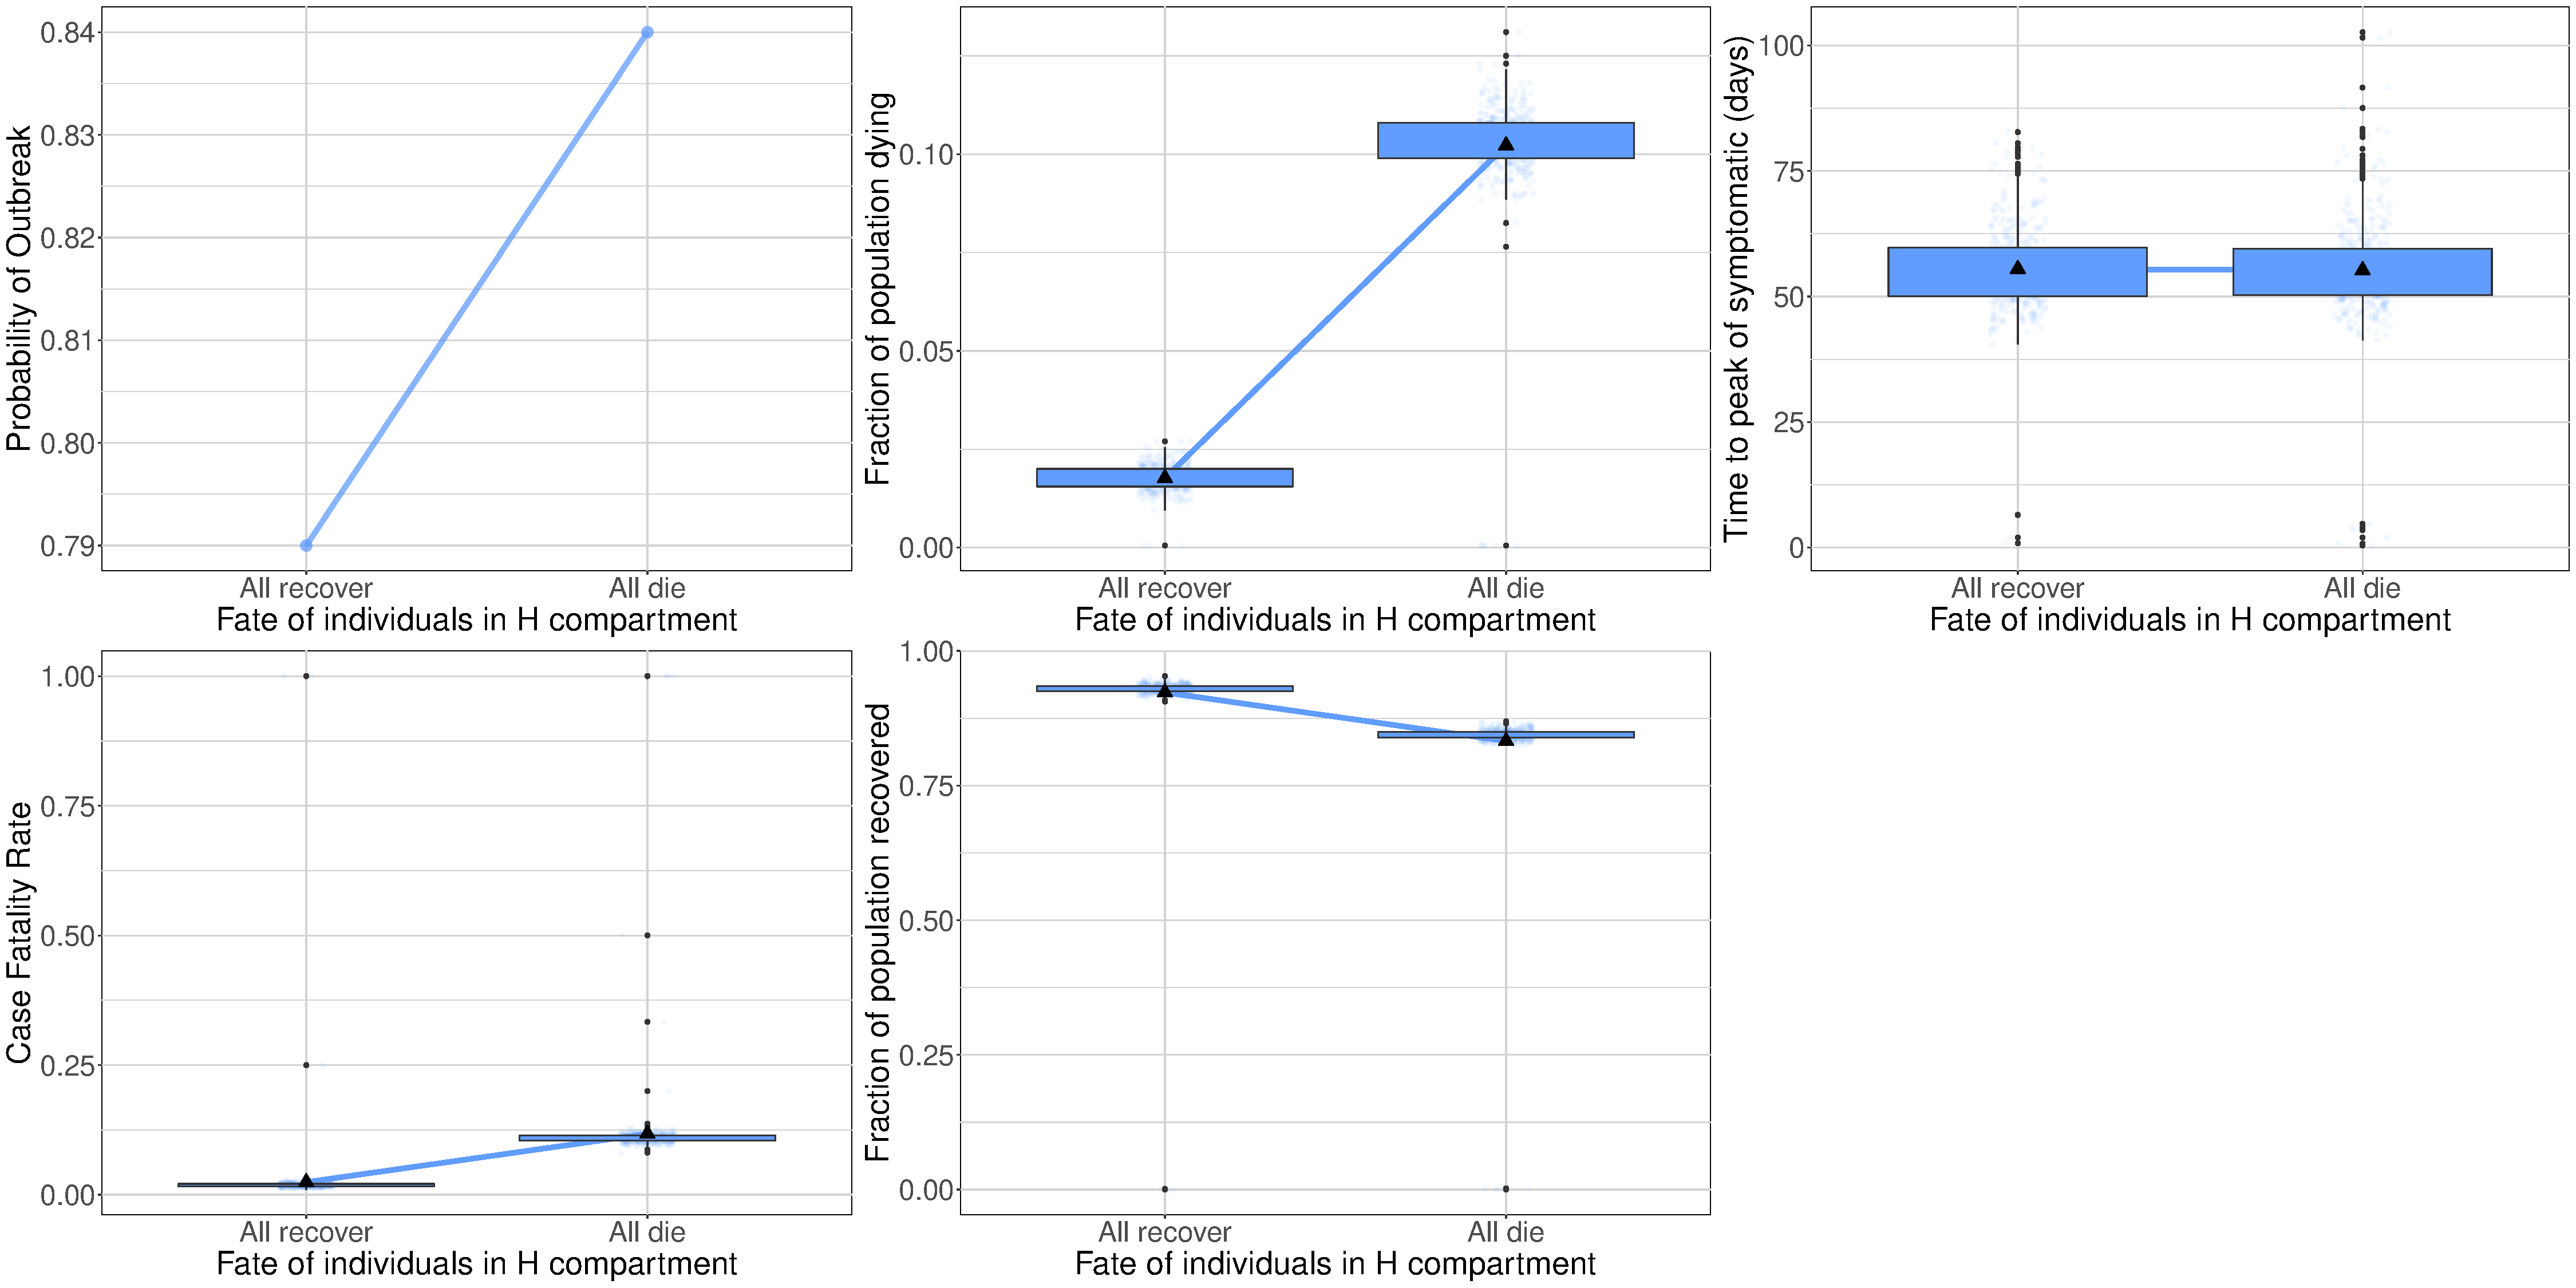
\includegraphics[width=1\textwidth]{figures/FigS2}\hspace{2mm}\caption{\label{fig:Suppl_DvsR} \textbf{Outcomes when all severe cases recover
vs when all severe cases die.} Probability of an outbreak (top left),
fraction of the population dying (top middle), time until peak symptomatic
cases (top right), CFR (bottom left), and fraction of the population
that recovers (bottom middle).}
\end{figure}

\medskip{}

\begin{figure}[H]
\centering{}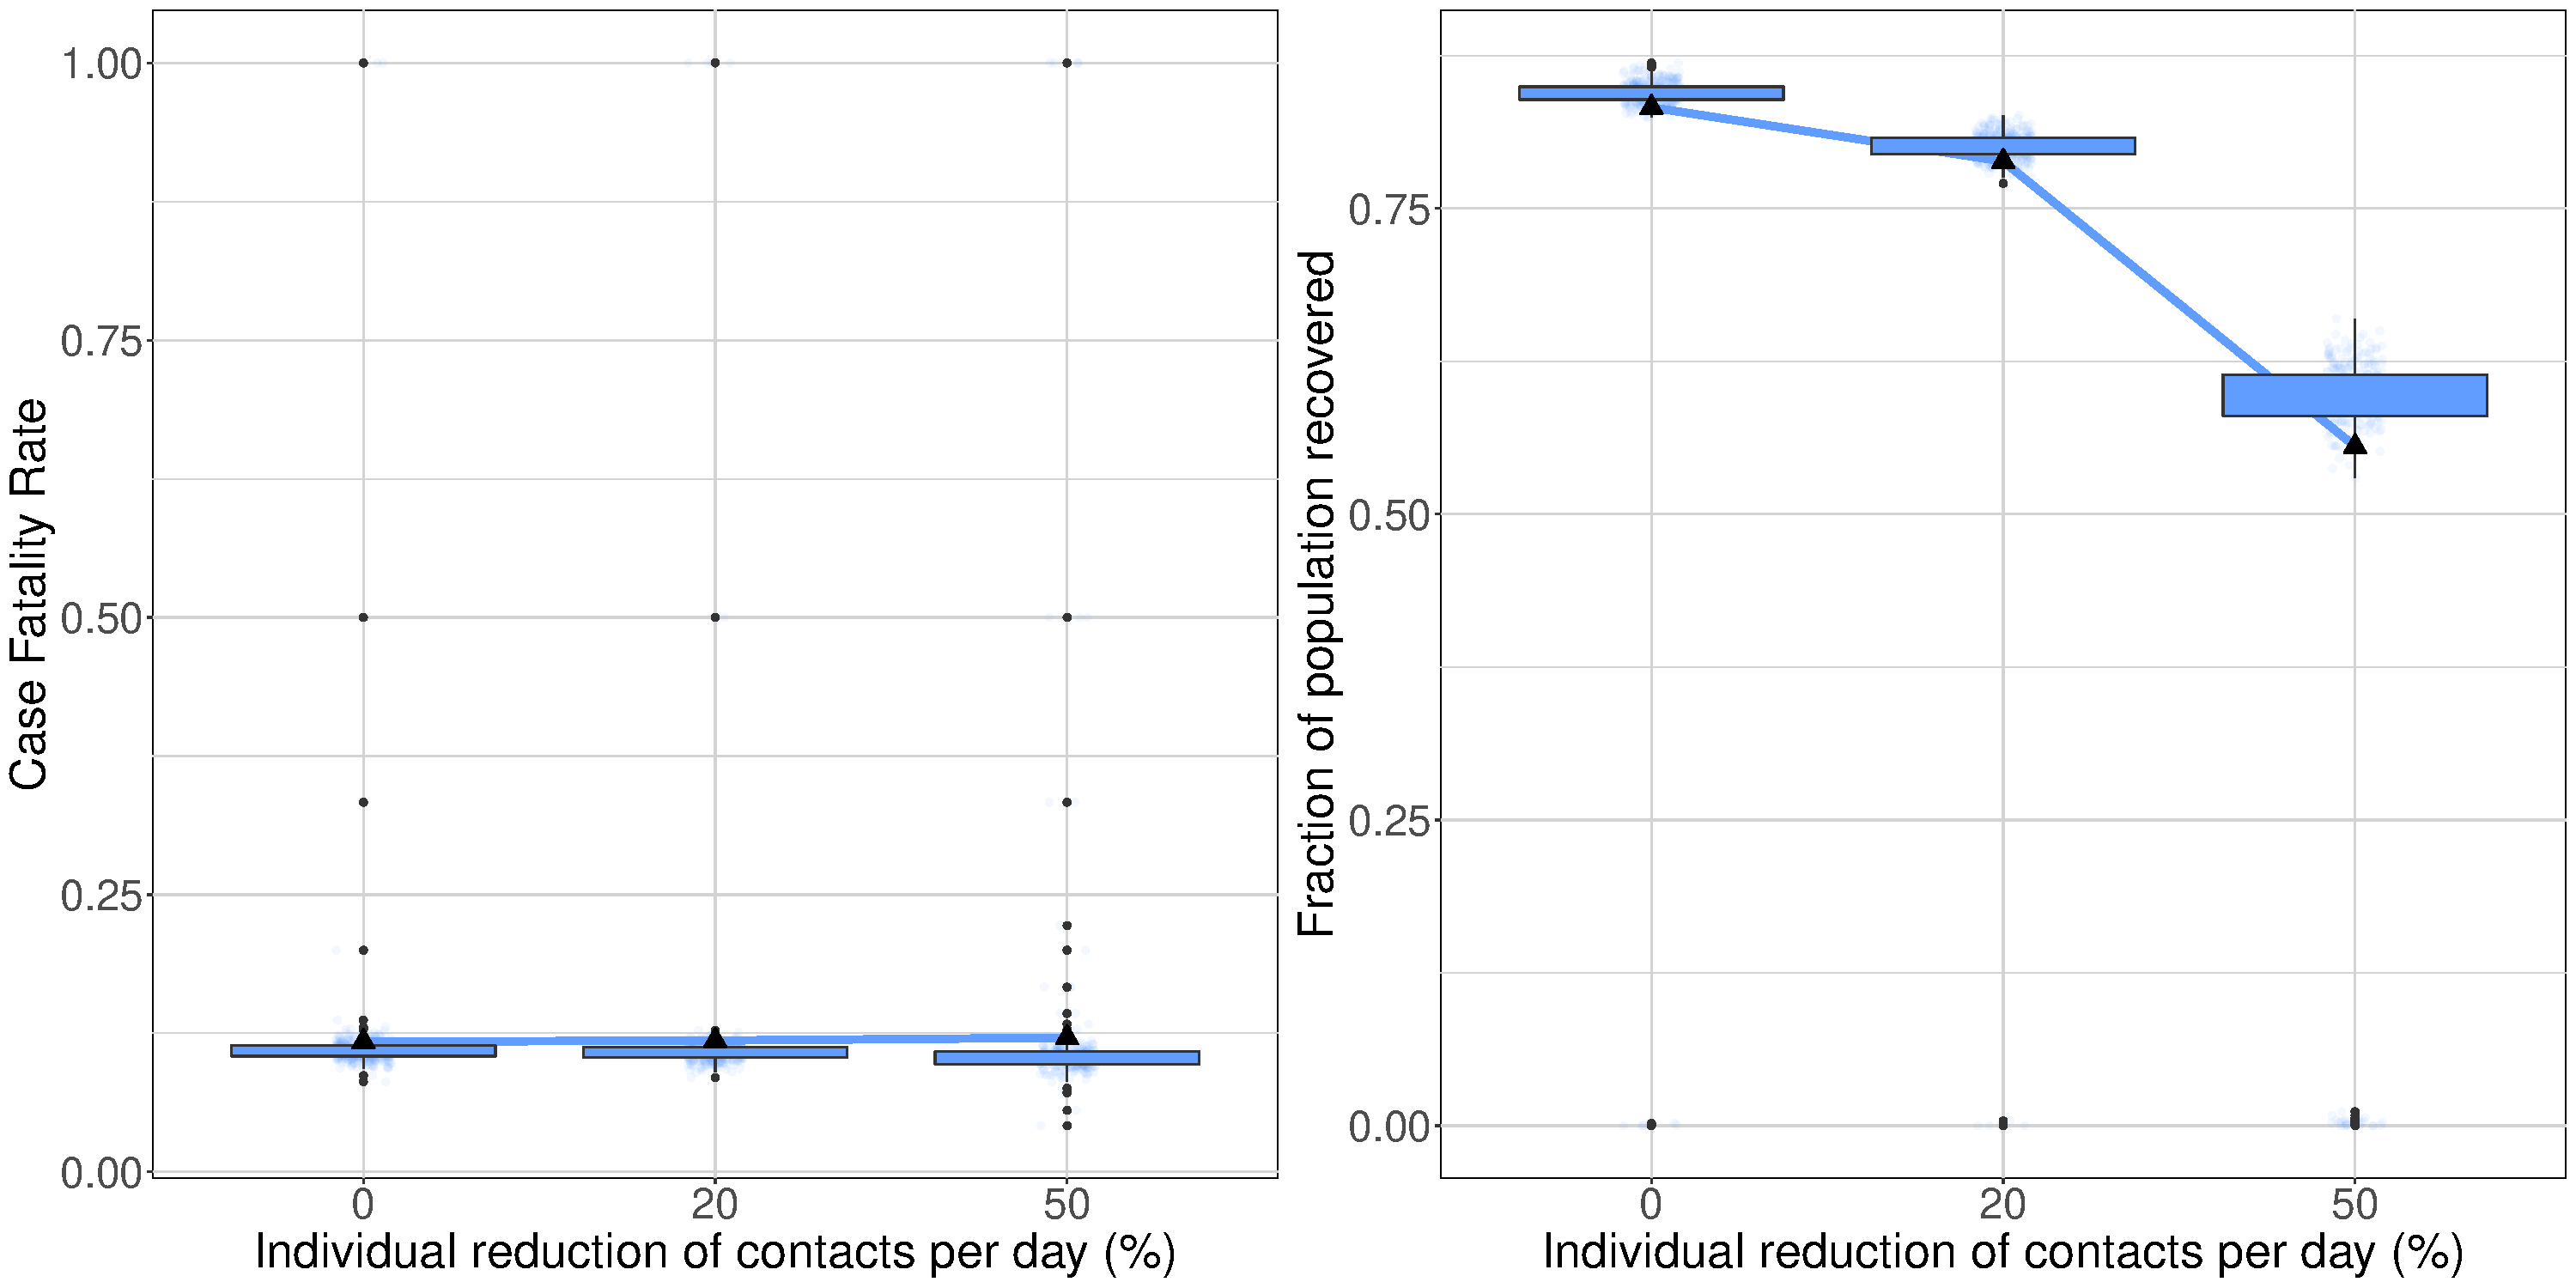
\includegraphics[width=1\textwidth]{figures/FigS3}\hspace{2mm}\caption{\label{fig:Suppl_self} \textbf{Self-distancing.} CFR (left), and
fraction of the population that recovers (right) as a function of
the proportion of contacts reduced per individual per day.}
\end{figure}
\medskip{}

\begin{figure}[H]
\centering{}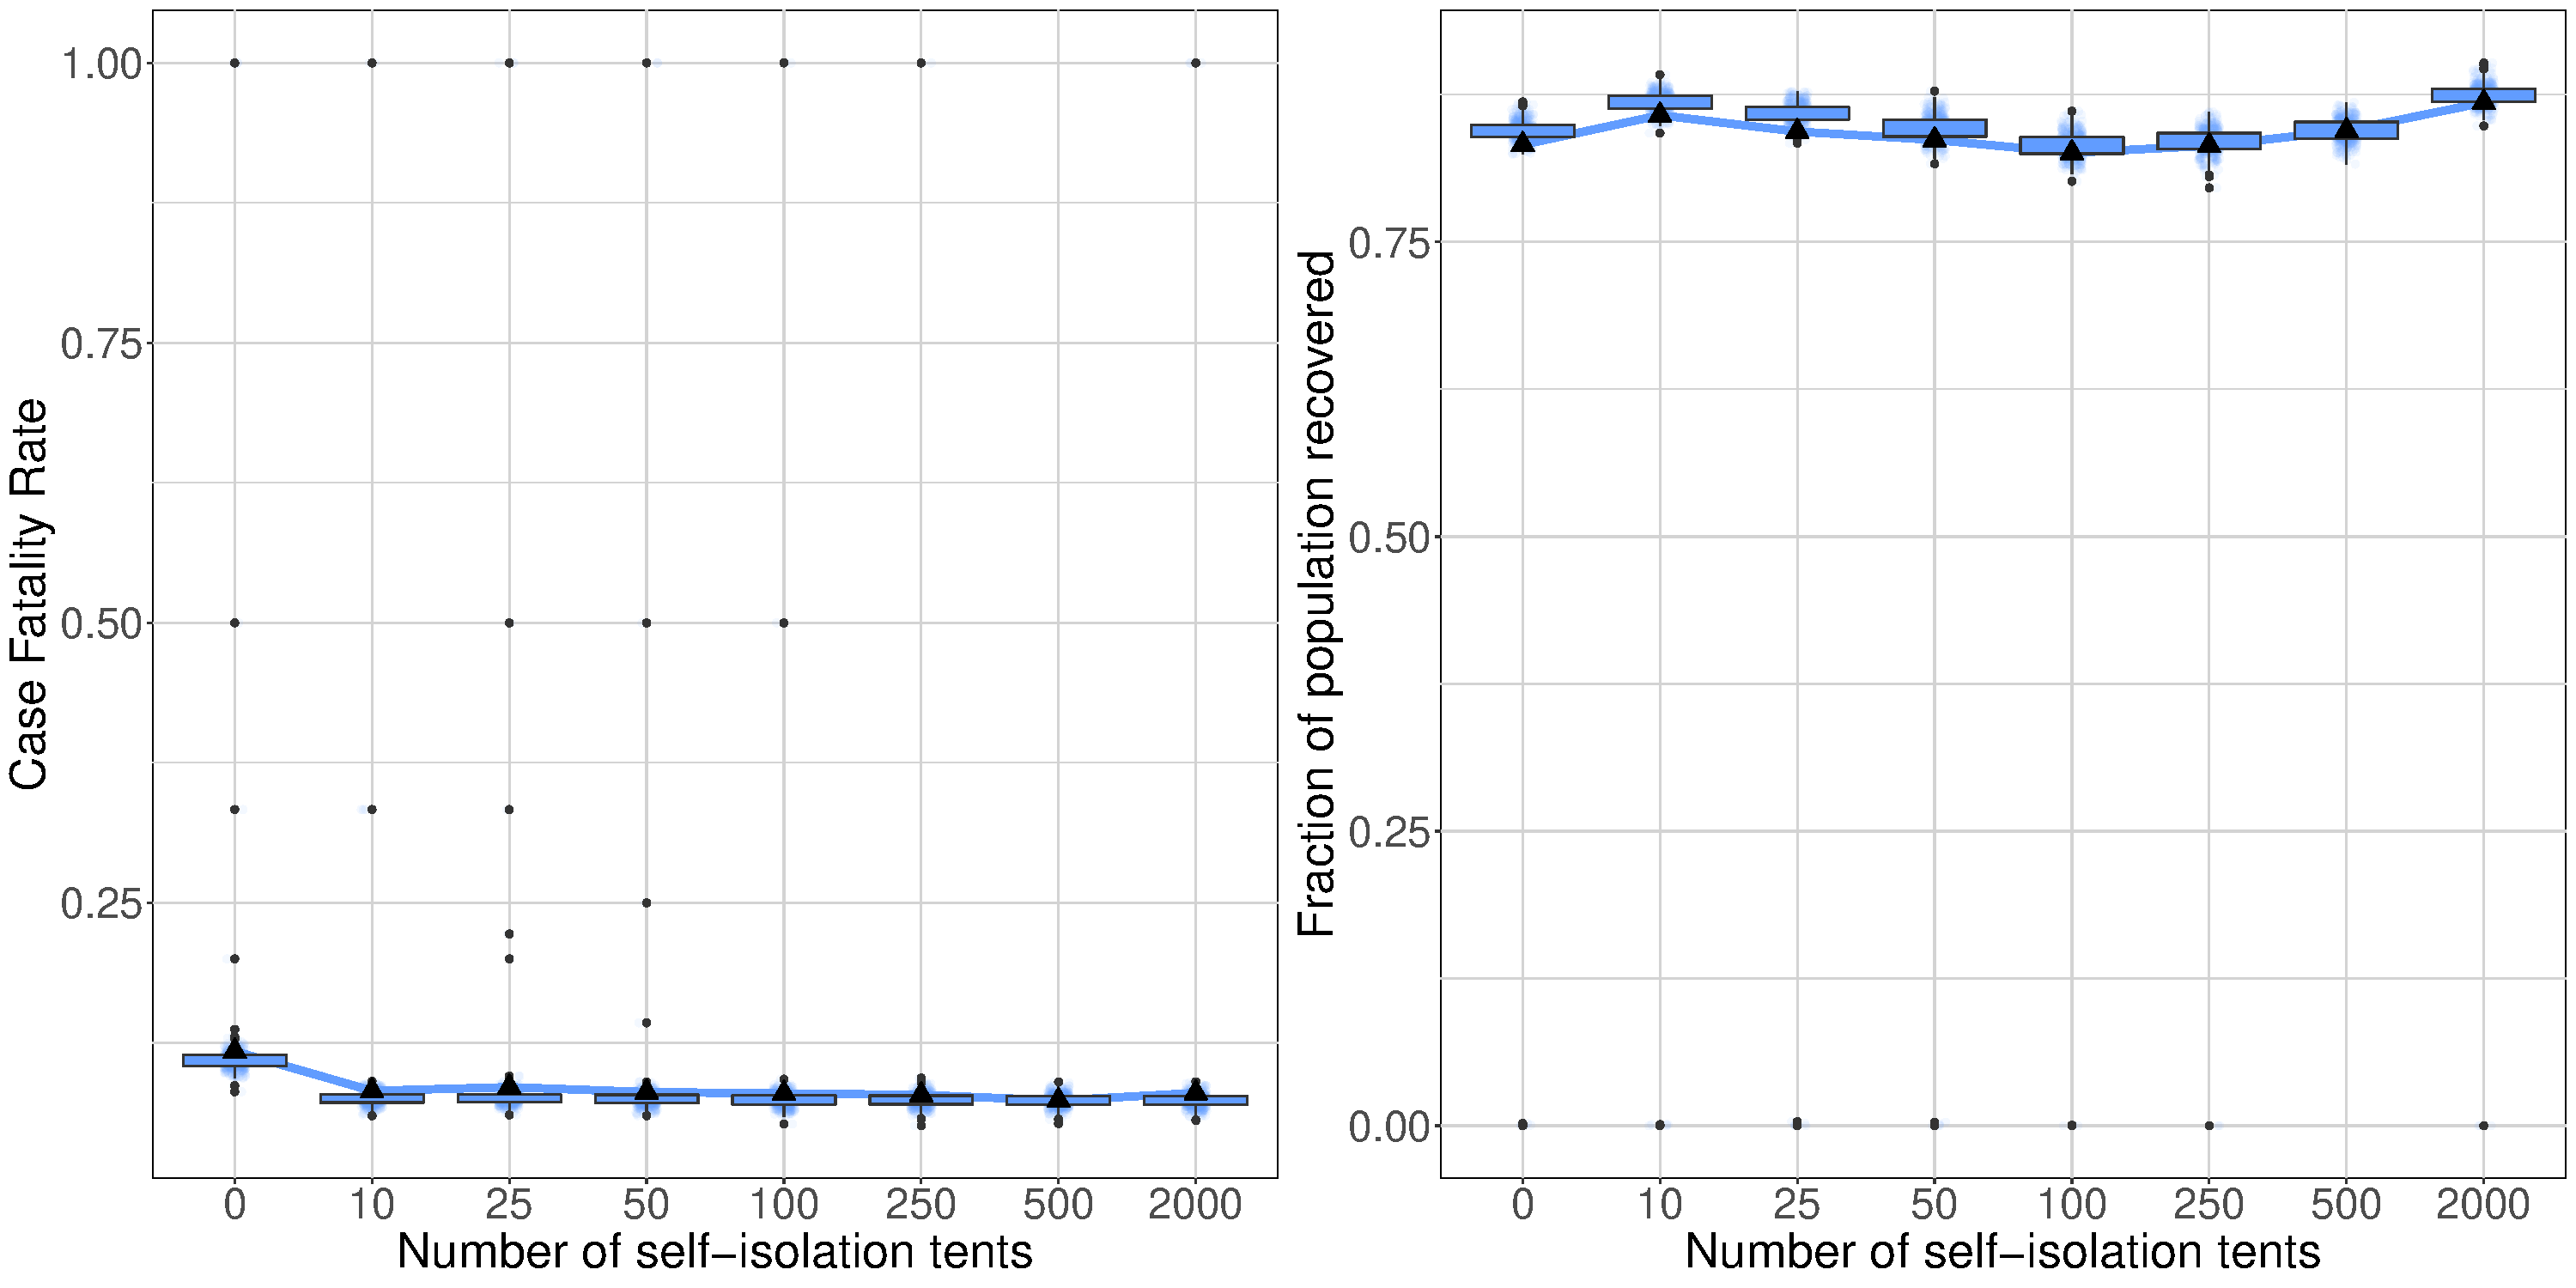
\includegraphics[width=1\textwidth]{figures/FigS4}\hspace{2mm}\caption{\label{fig:Suppl_isolation} \textbf{Self-isolation.} CFR (left),
and fraction of the population that recovers (right) as a function
of the number of isolation tents available in the camp.}
\end{figure}

\medskip{}

\begin{figure}[H]
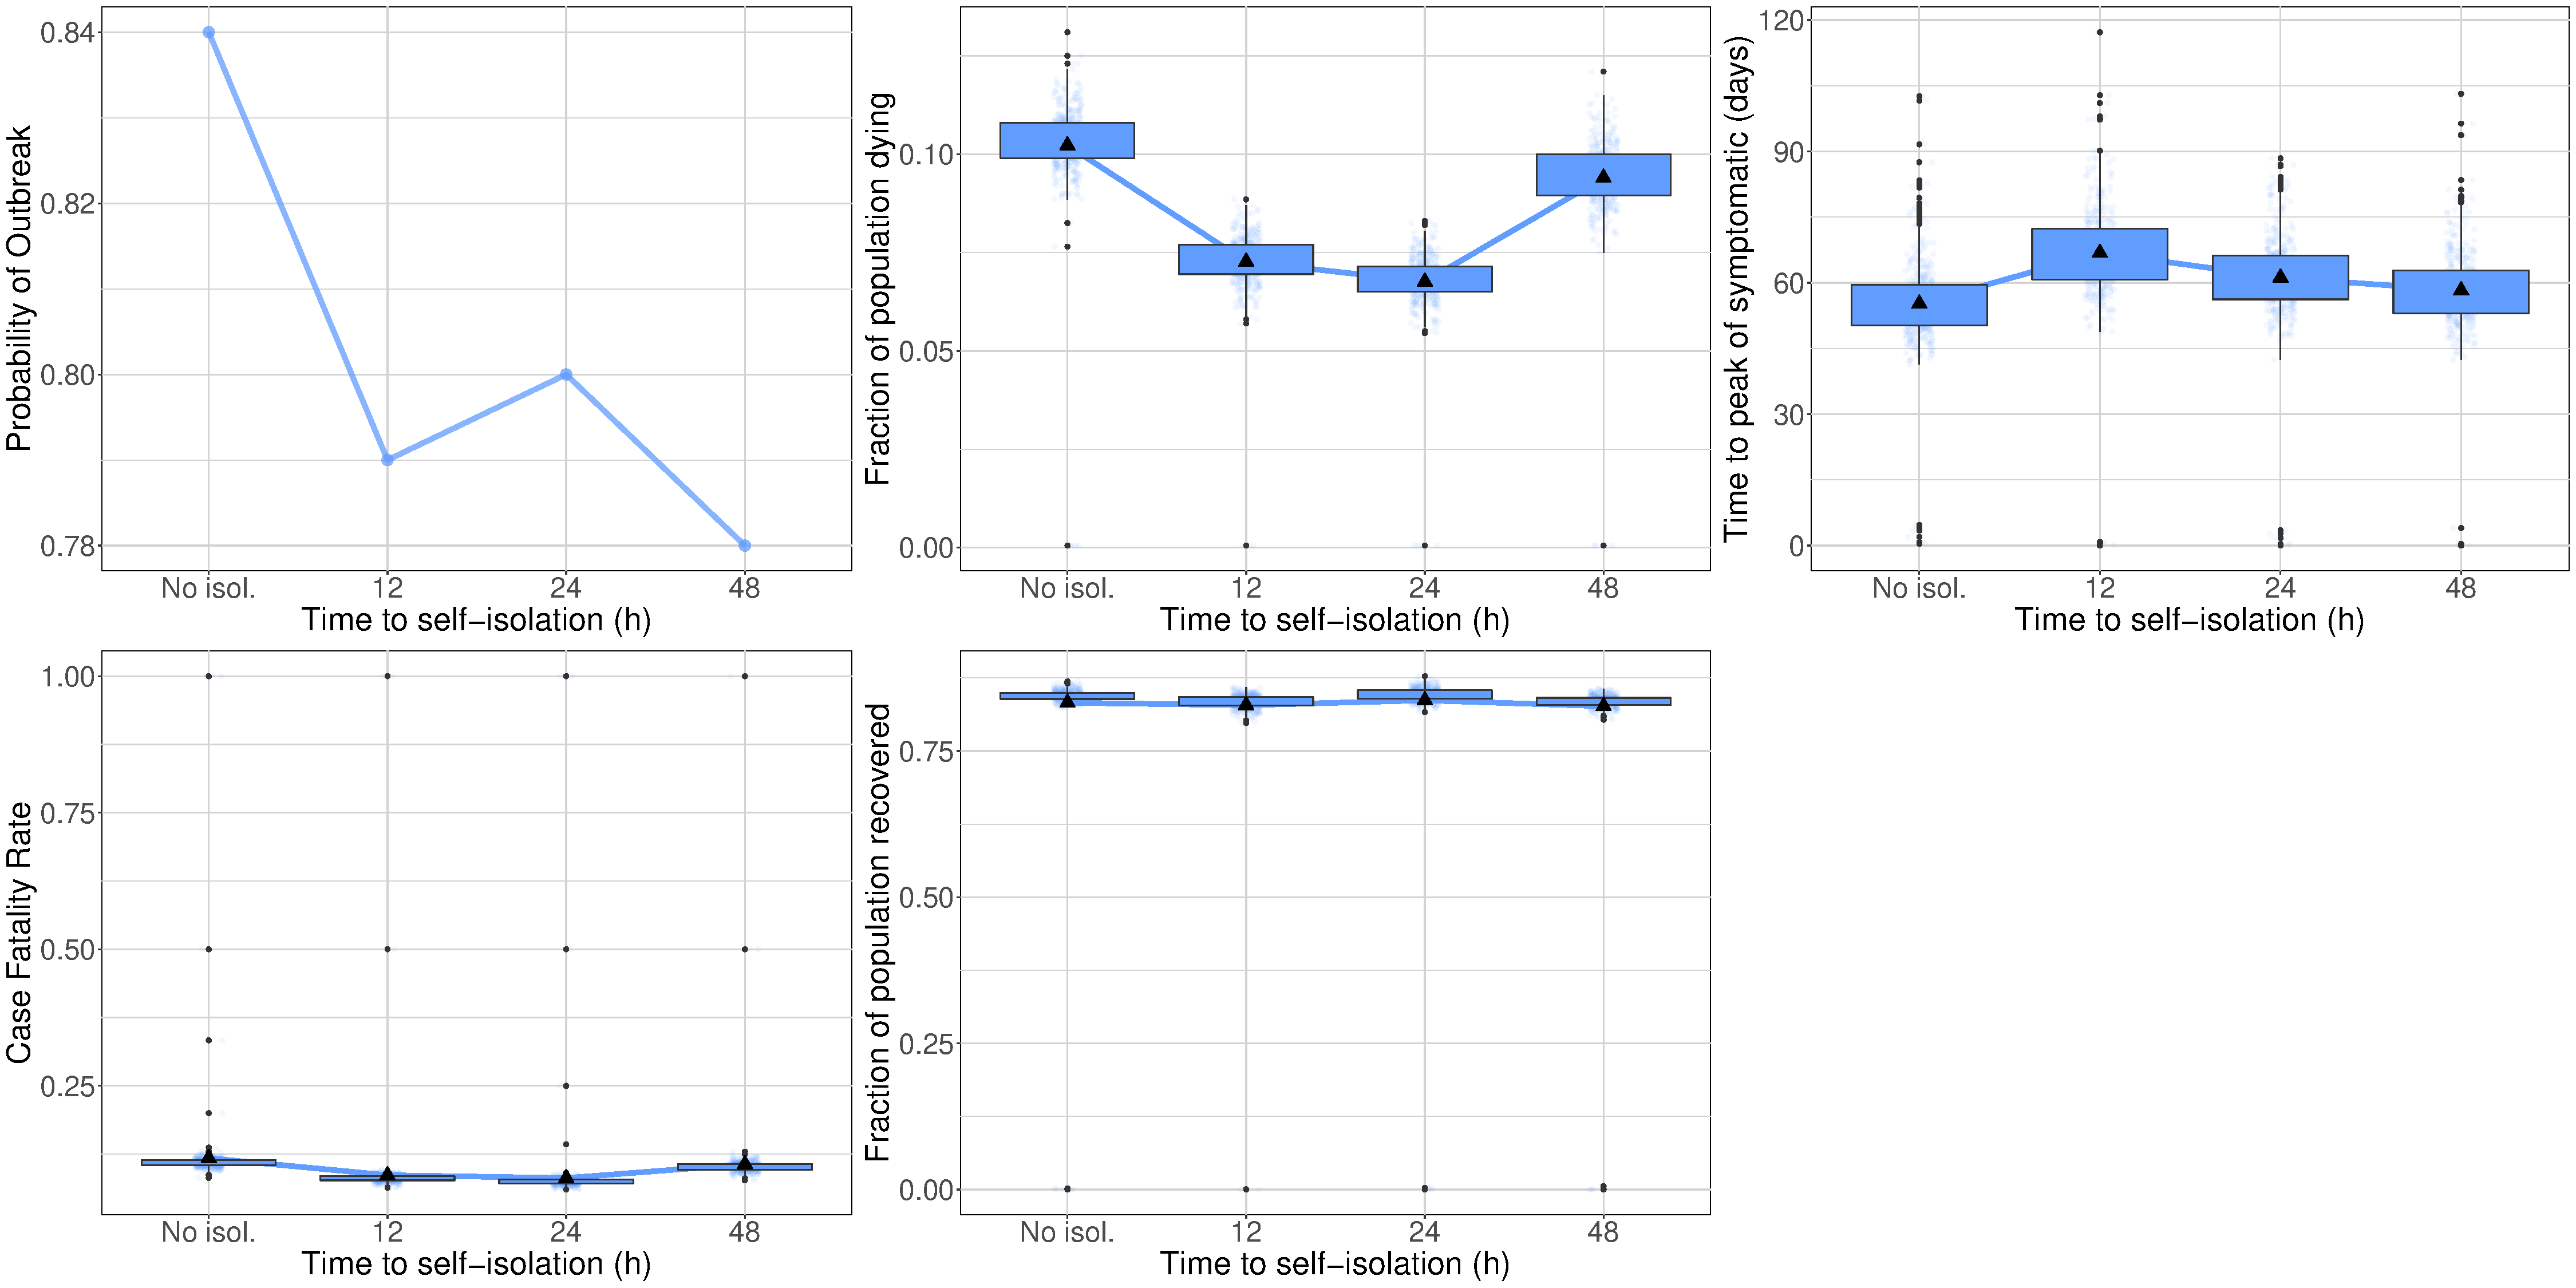
\includegraphics[width=1\textwidth]{figures/FigS5}\hspace{2mm}\caption{\label{fig:Suppl_onset} \textbf{Time to self-isolation.} Probability
of an outbreak (top left), fraction of the population dying (top middle),
time until peak symptomatic cases (top right), CFR (bottom left),
and fraction of the population that recovers (bottom middle) as a
function of the time that individuals require to recognize their symptoms
and self-isolate.}
\end{figure}

\medskip{}

\begin{figure}[H]
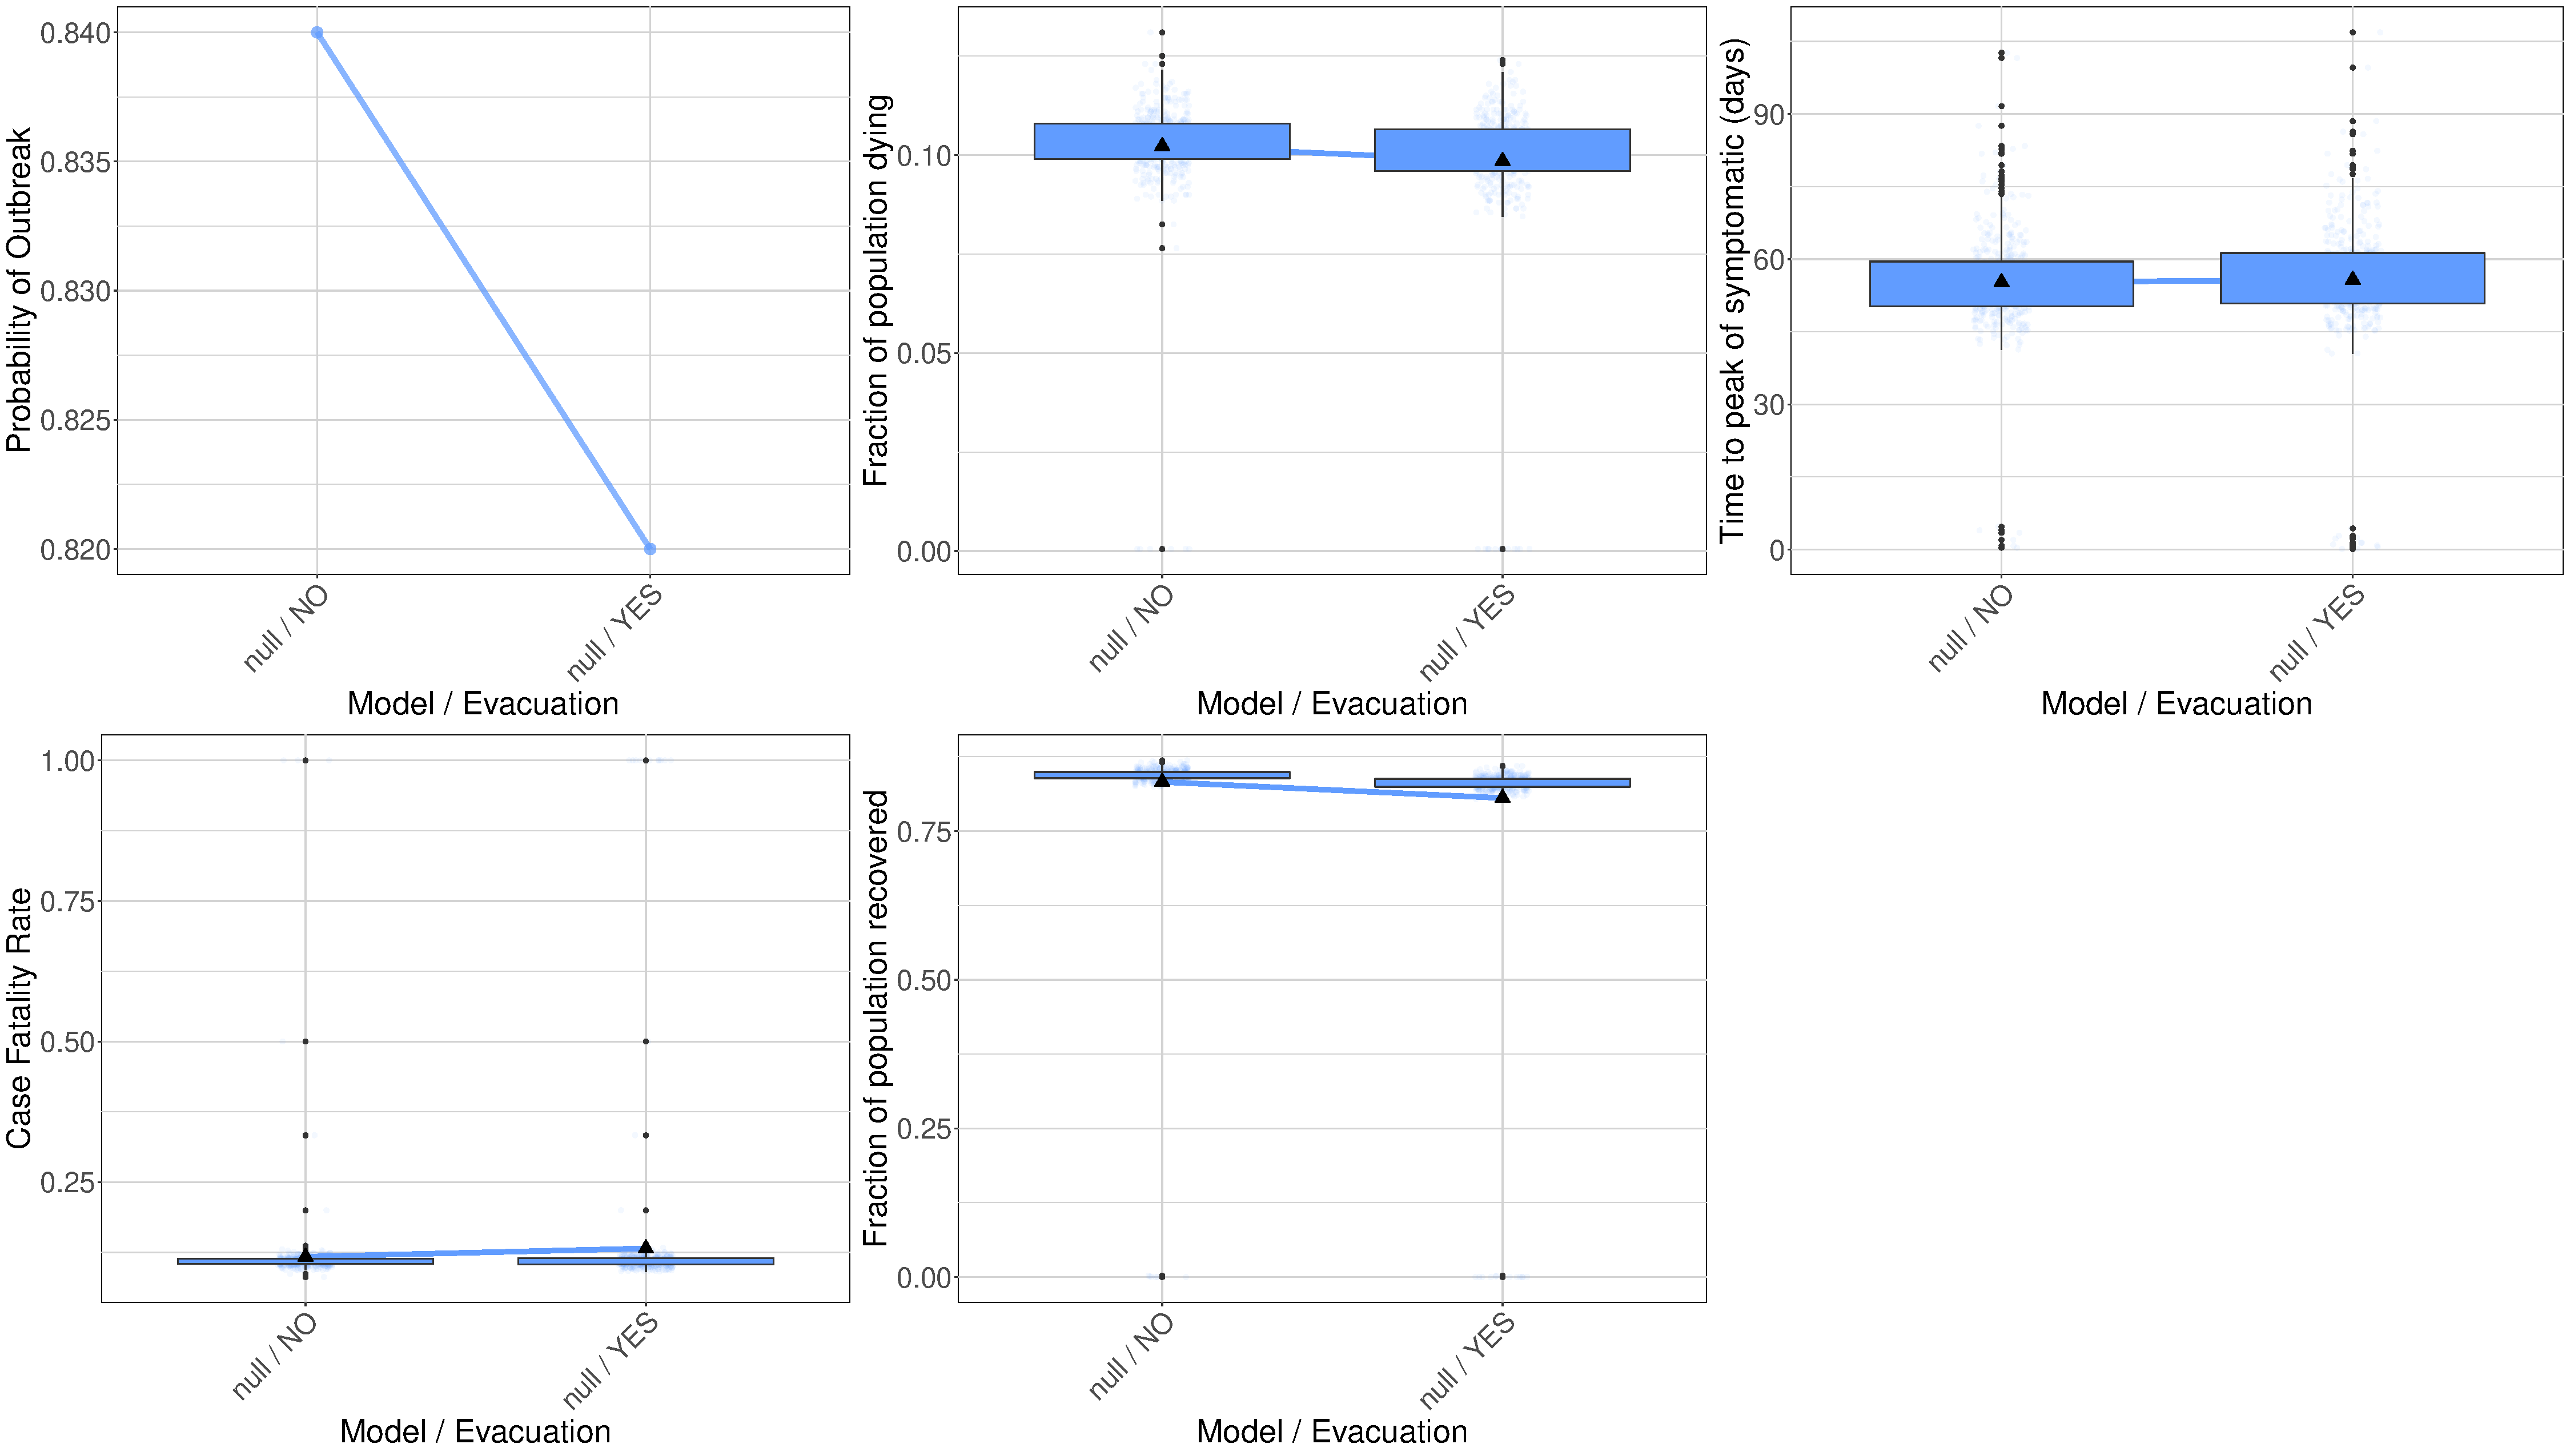
\includegraphics[width=1\textwidth]{figures/FigS6}\hspace{2mm}\caption{\label{fig:Suppl_evacuation} \textbf{Evacuation.} Probability of
an outbreak (top left), fraction of the population dying (top middle),
time until peak symptomatic cases (top right), CFR (bottom left),
and fraction of the population that recovers (bottom middle), as a
function of whether individuals requiring hospitalization are evacuated
to isolation centers.}
\end{figure}

\medskip{}

\begin{figure}[H]
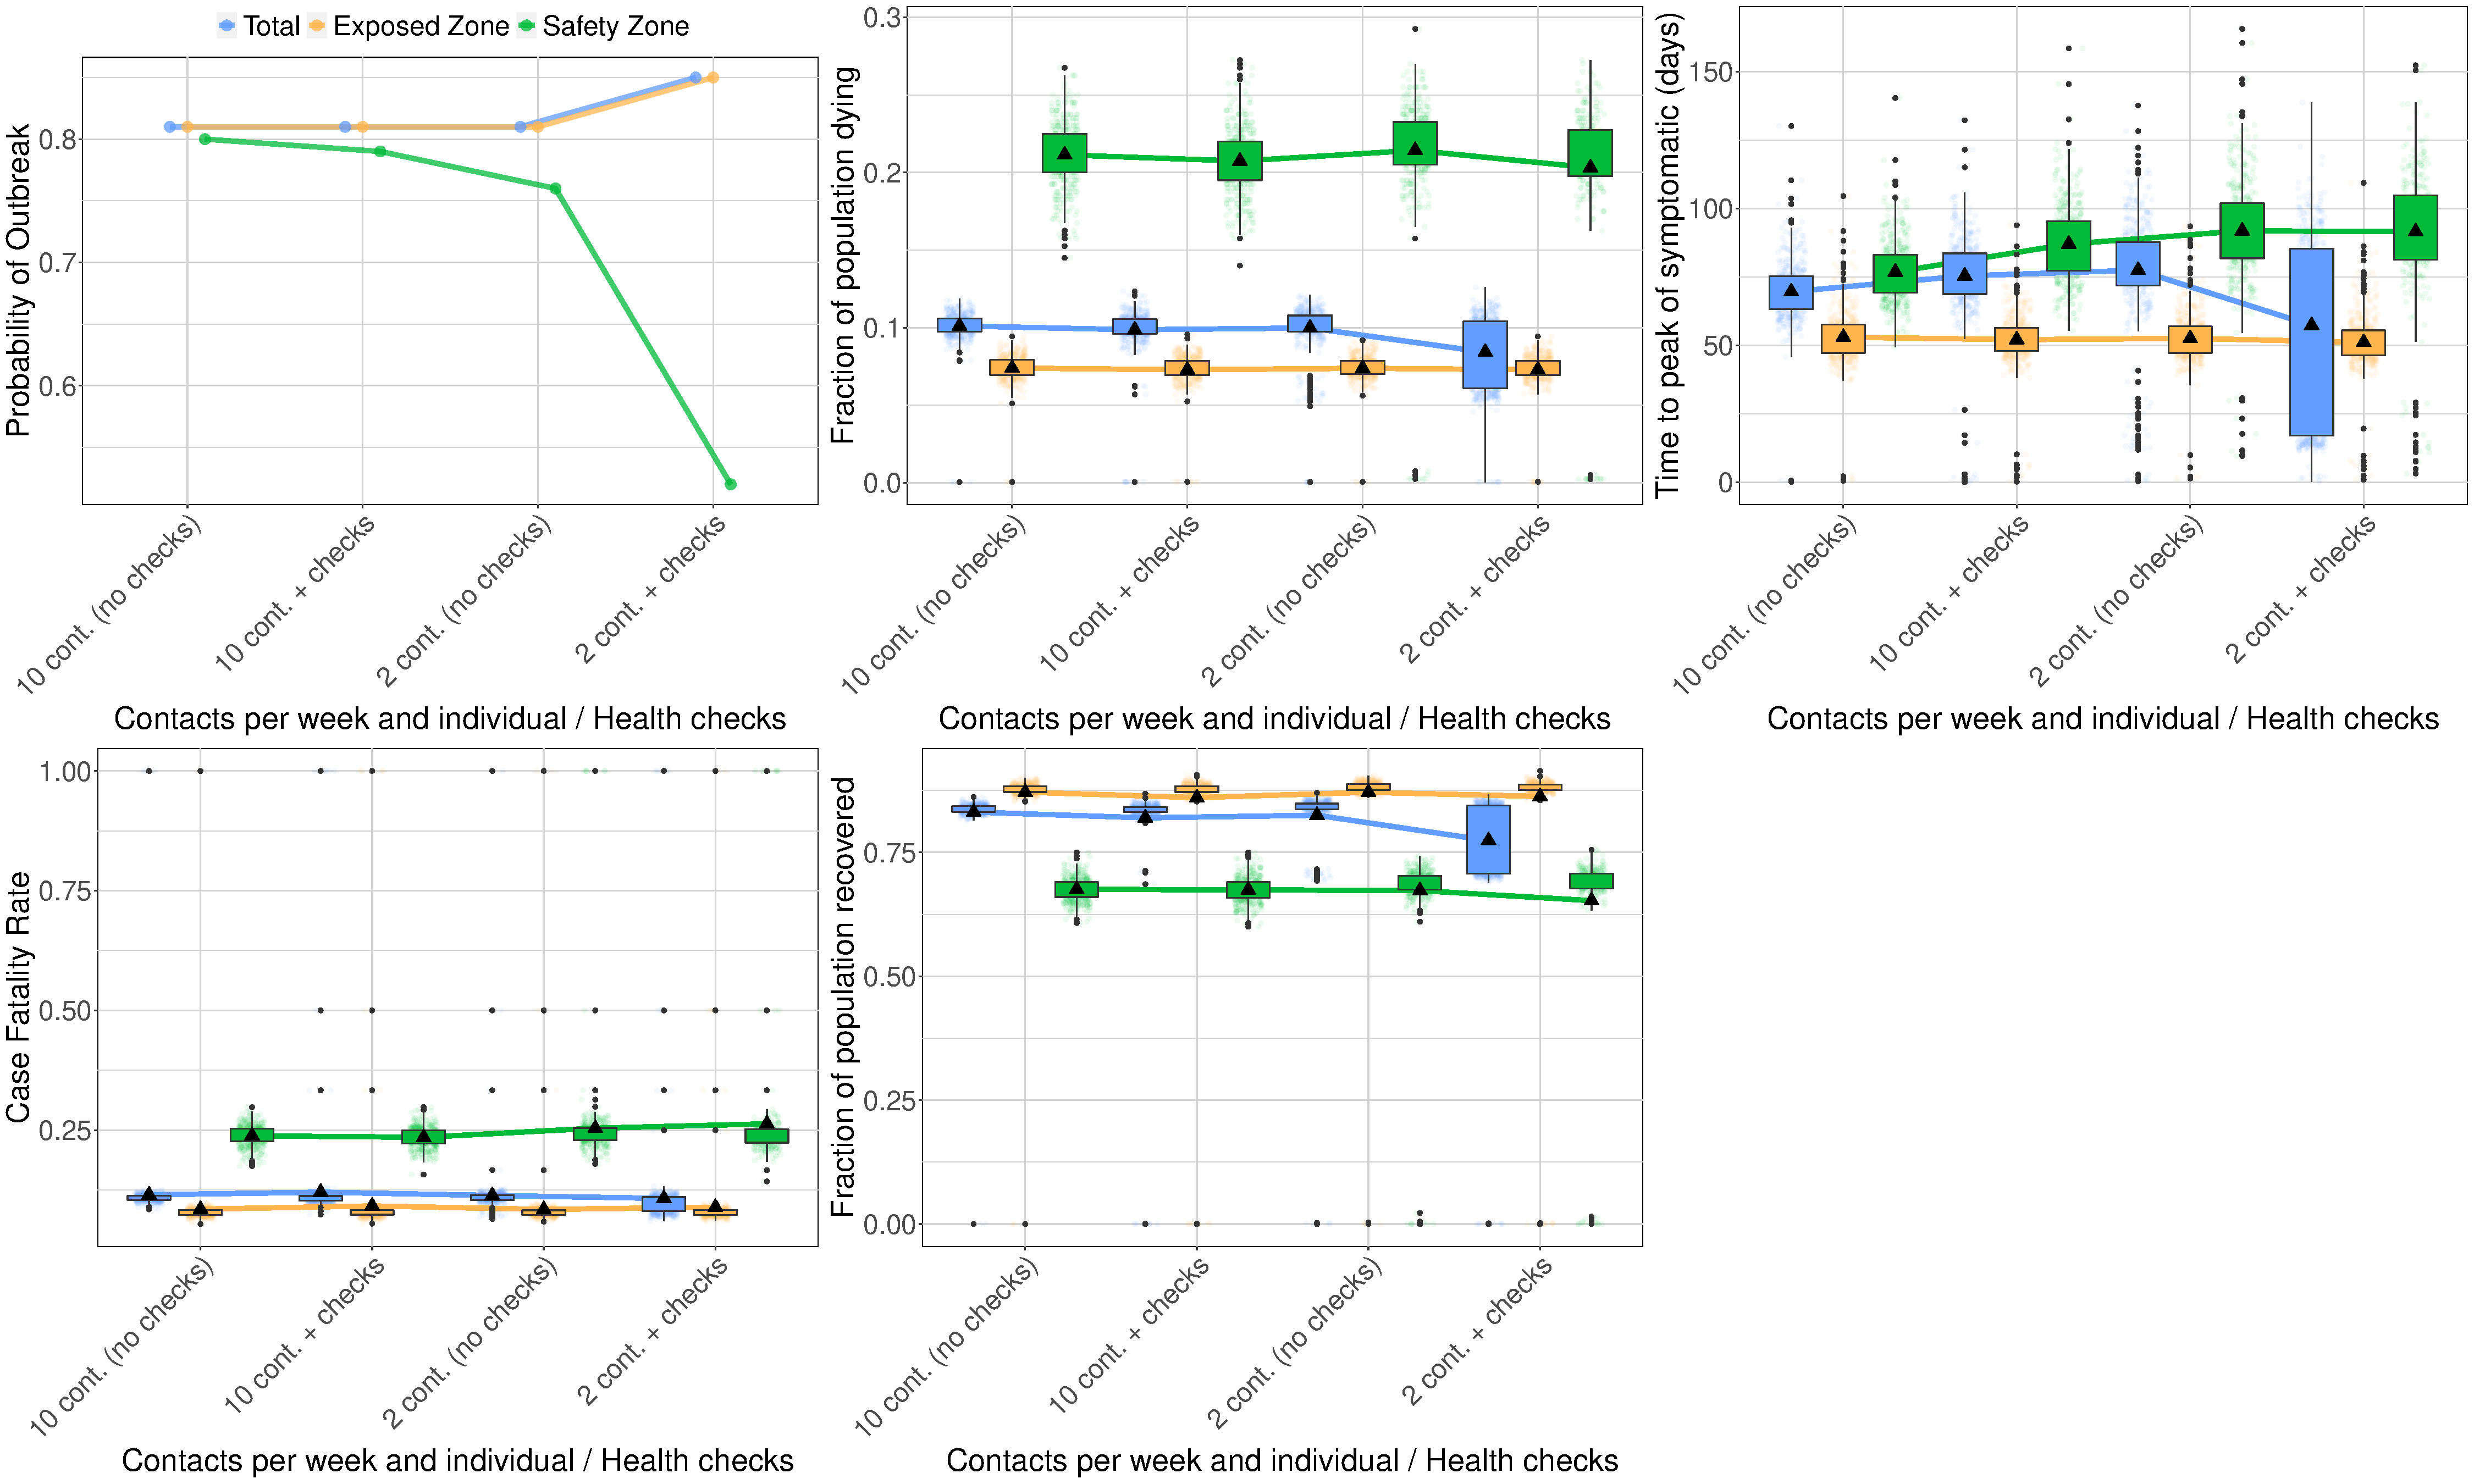
\includegraphics[width=1\textwidth]{figures/FigS7}\hspace{2mm}\caption{\label{fig:Suppl_Tcheck} \textbf{Health-checks in the buffer zone.}
Probability of an outbreak (top left), fraction of the population
dying (top middle), time until peak symptomatic cases (top right),
CFR (bottom left), and fraction of the population that recovers (bottom
middle), as a function of whether health-checks are implemented in
the buffer zone between the safety and exposed zones. Scenarios with
10 or 2 contacts in the buffer zone per person in the safety zone
per week are plotted. All figures consider the scenario in which 20\%
of the camp's population is allocated to the safety zone.}
\end{figure}

\begin{figure}[H]
\centering{}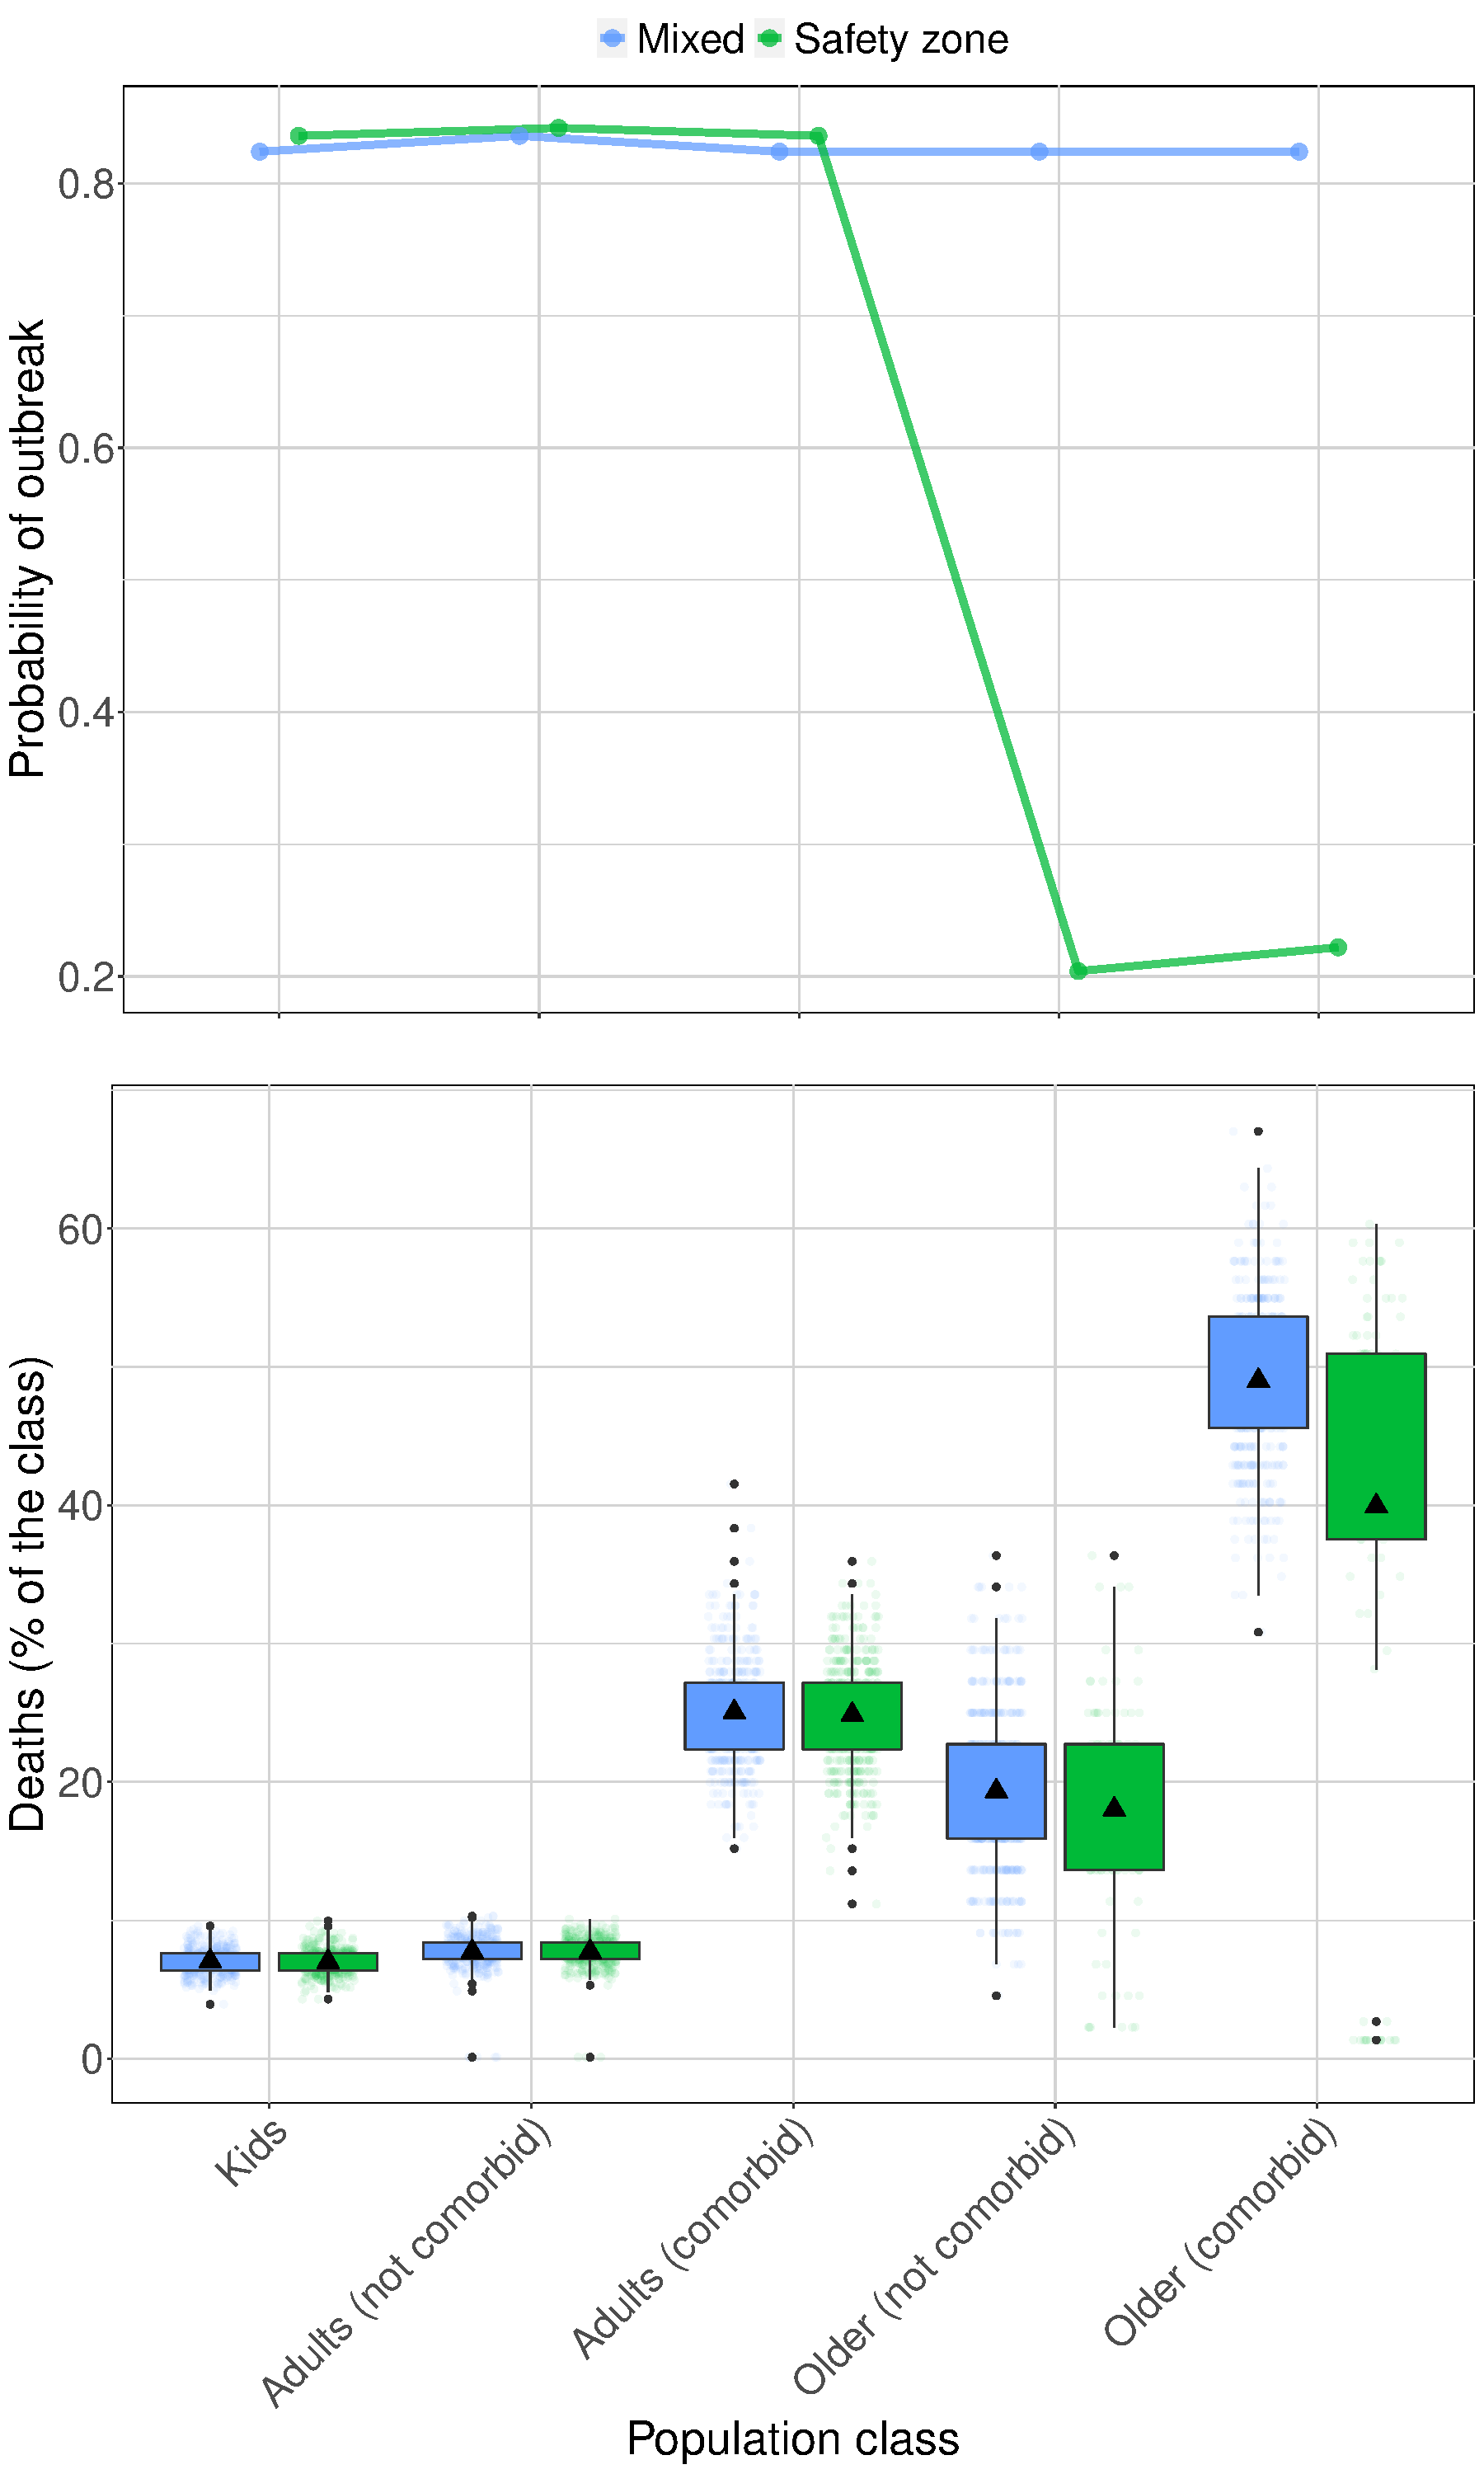
\includegraphics[width=0.6\textwidth]{figures/FigS8}\hspace{2mm}\caption{\label{fig:Suppl_agegroups} \textbf{Effects of the safety zone on
outcomes by population class. }Probability of an outbreak (top), and
proportion that dies in each population class (bottom) when no interventions
are implemented (Mixed), compared to protection of older adults in
the safety zone with 2 contacts in the buffer zone per week (Safety
zone). The fraction of deaths in the safety zone for the older population
is significantly lower (Kruskal-Wallis test, p-val$<10^{-15}$).}
\end{figure}
\medskip{}

\begin{figure}[H]
\centering{}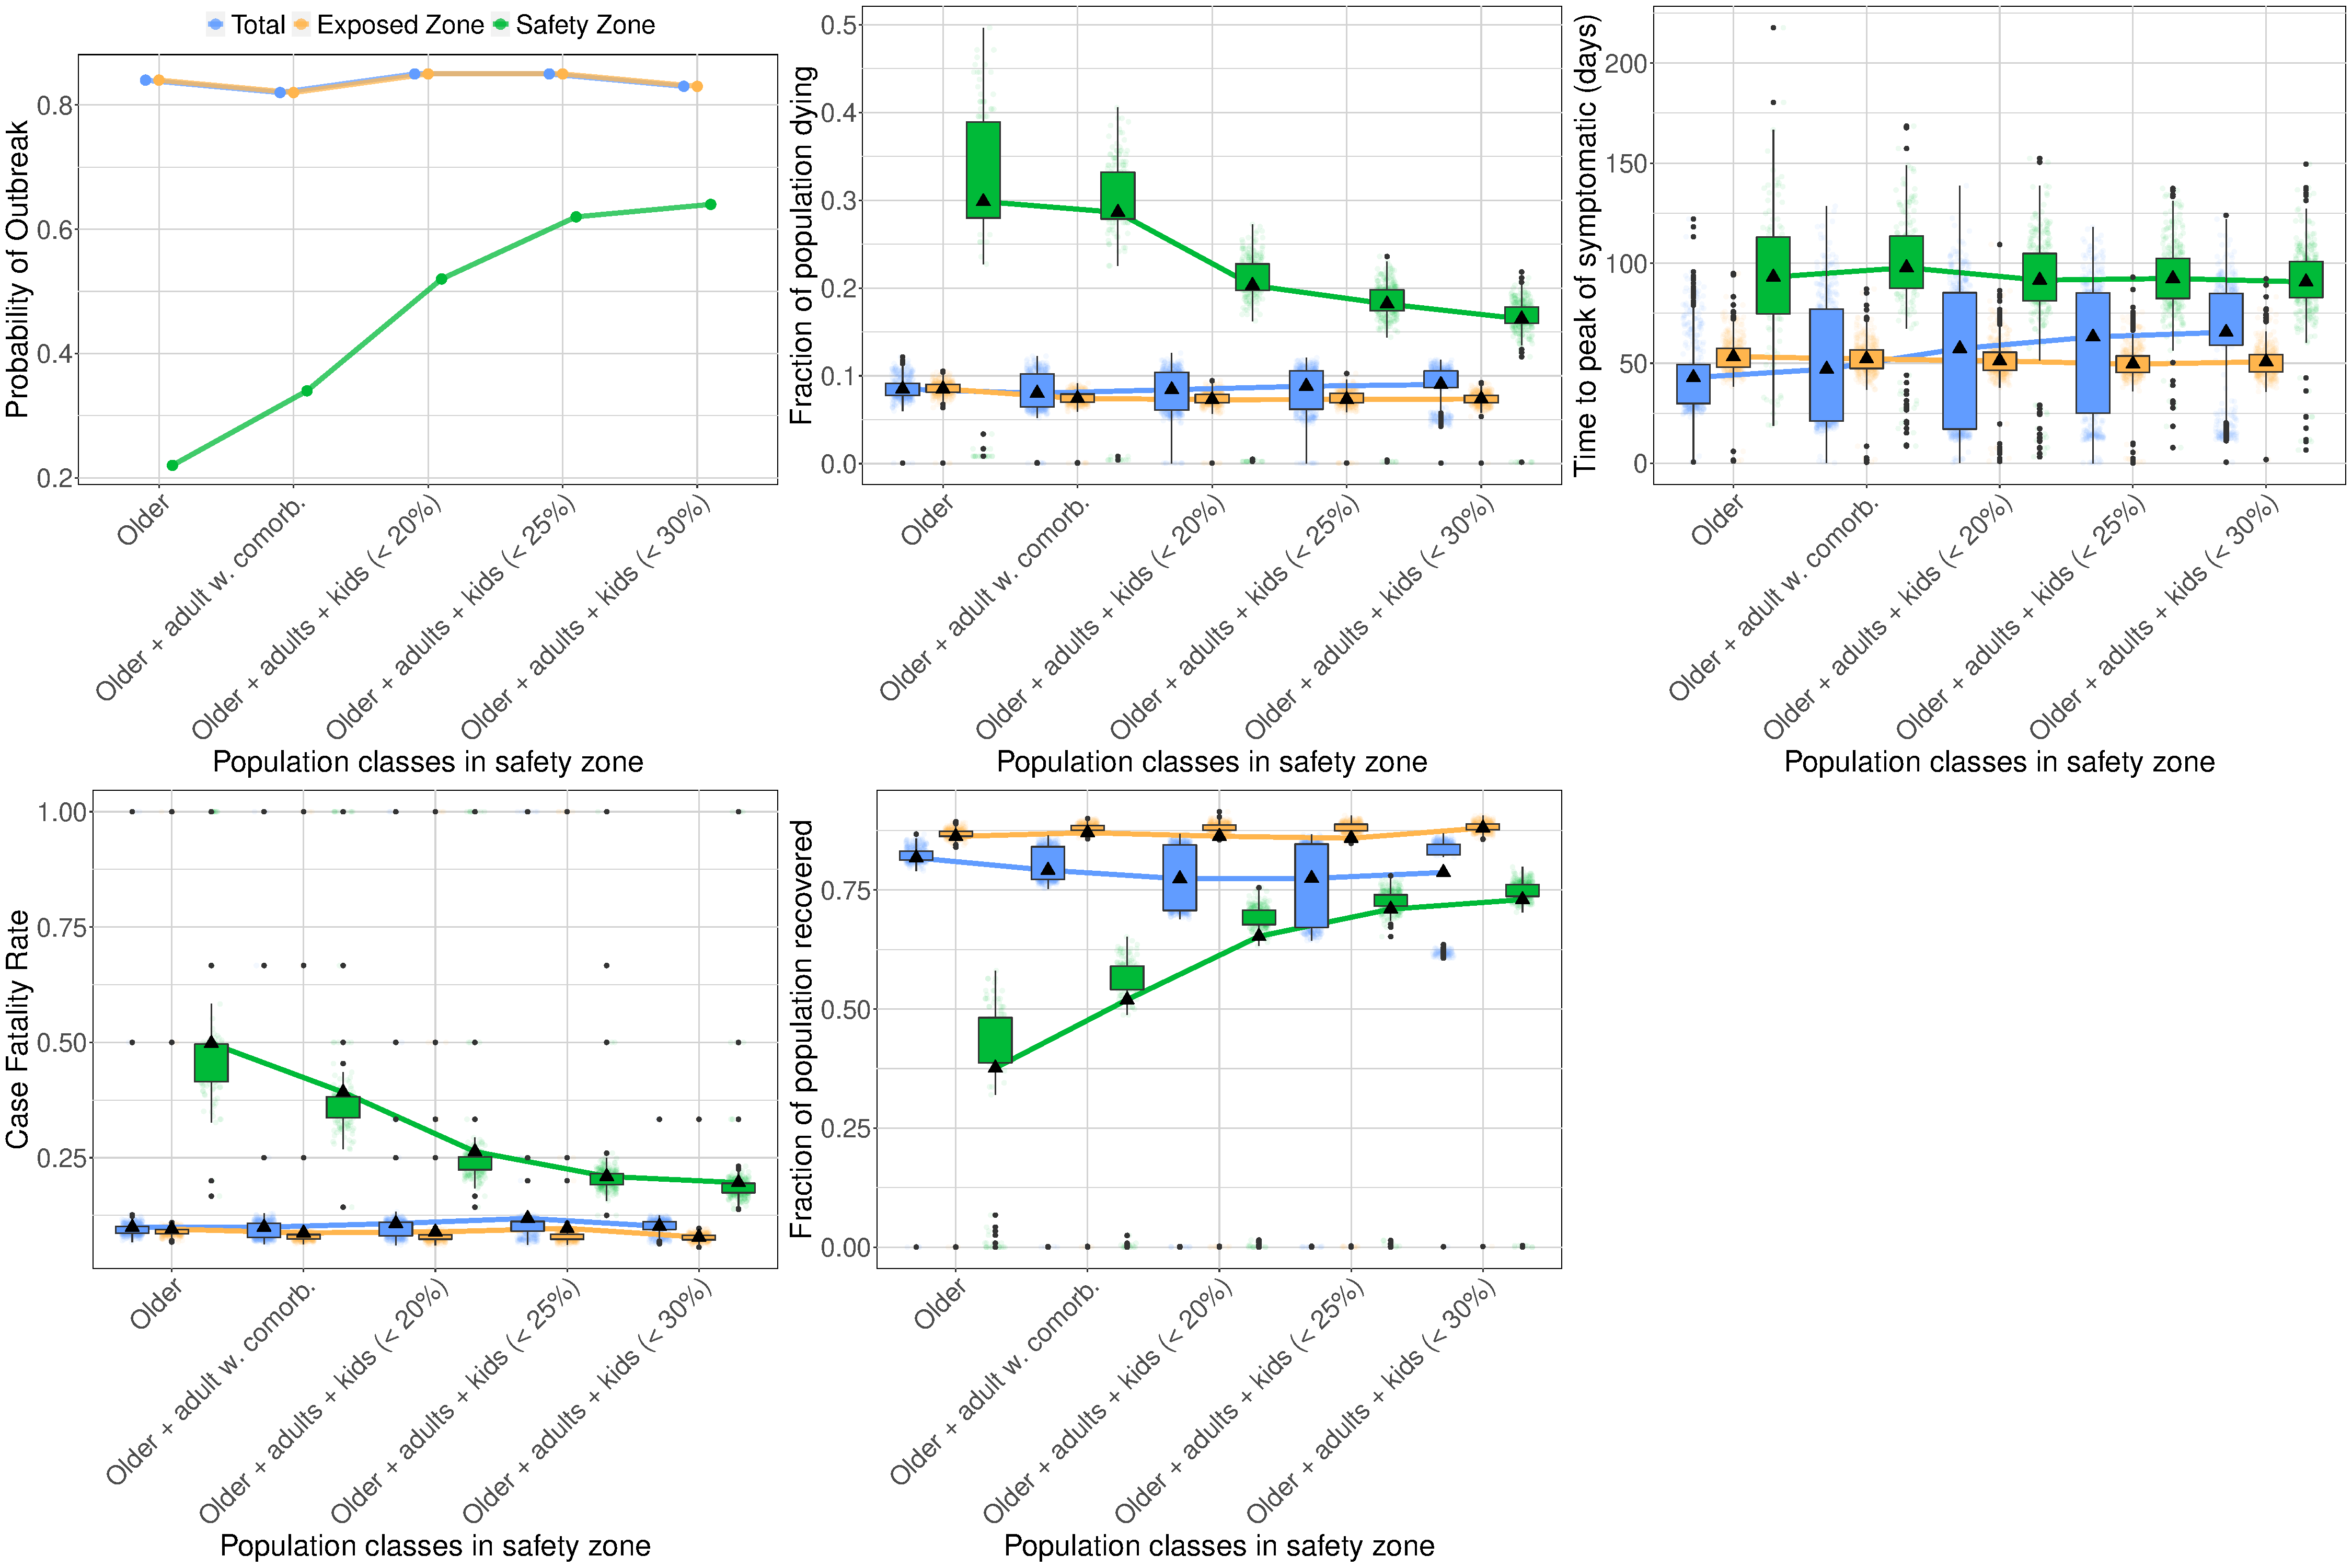
\includegraphics[width=1\textwidth]{figures/FigS9}\hspace{2mm}\caption{\label{fig:Suppl_safety} \textbf{Number of contacts in the buffer
zone.} CFR (left), and fraction of the population that recovers (right)
as a function of the number of contacts that each individual in the
safety zone has in the buffer zone per week. All figures consider
the scenario in which 20\% of the camp's population is allocated to
the safety zone.}
\end{figure}
\medskip{}

\begin{figure}[H]
\begin{centering}
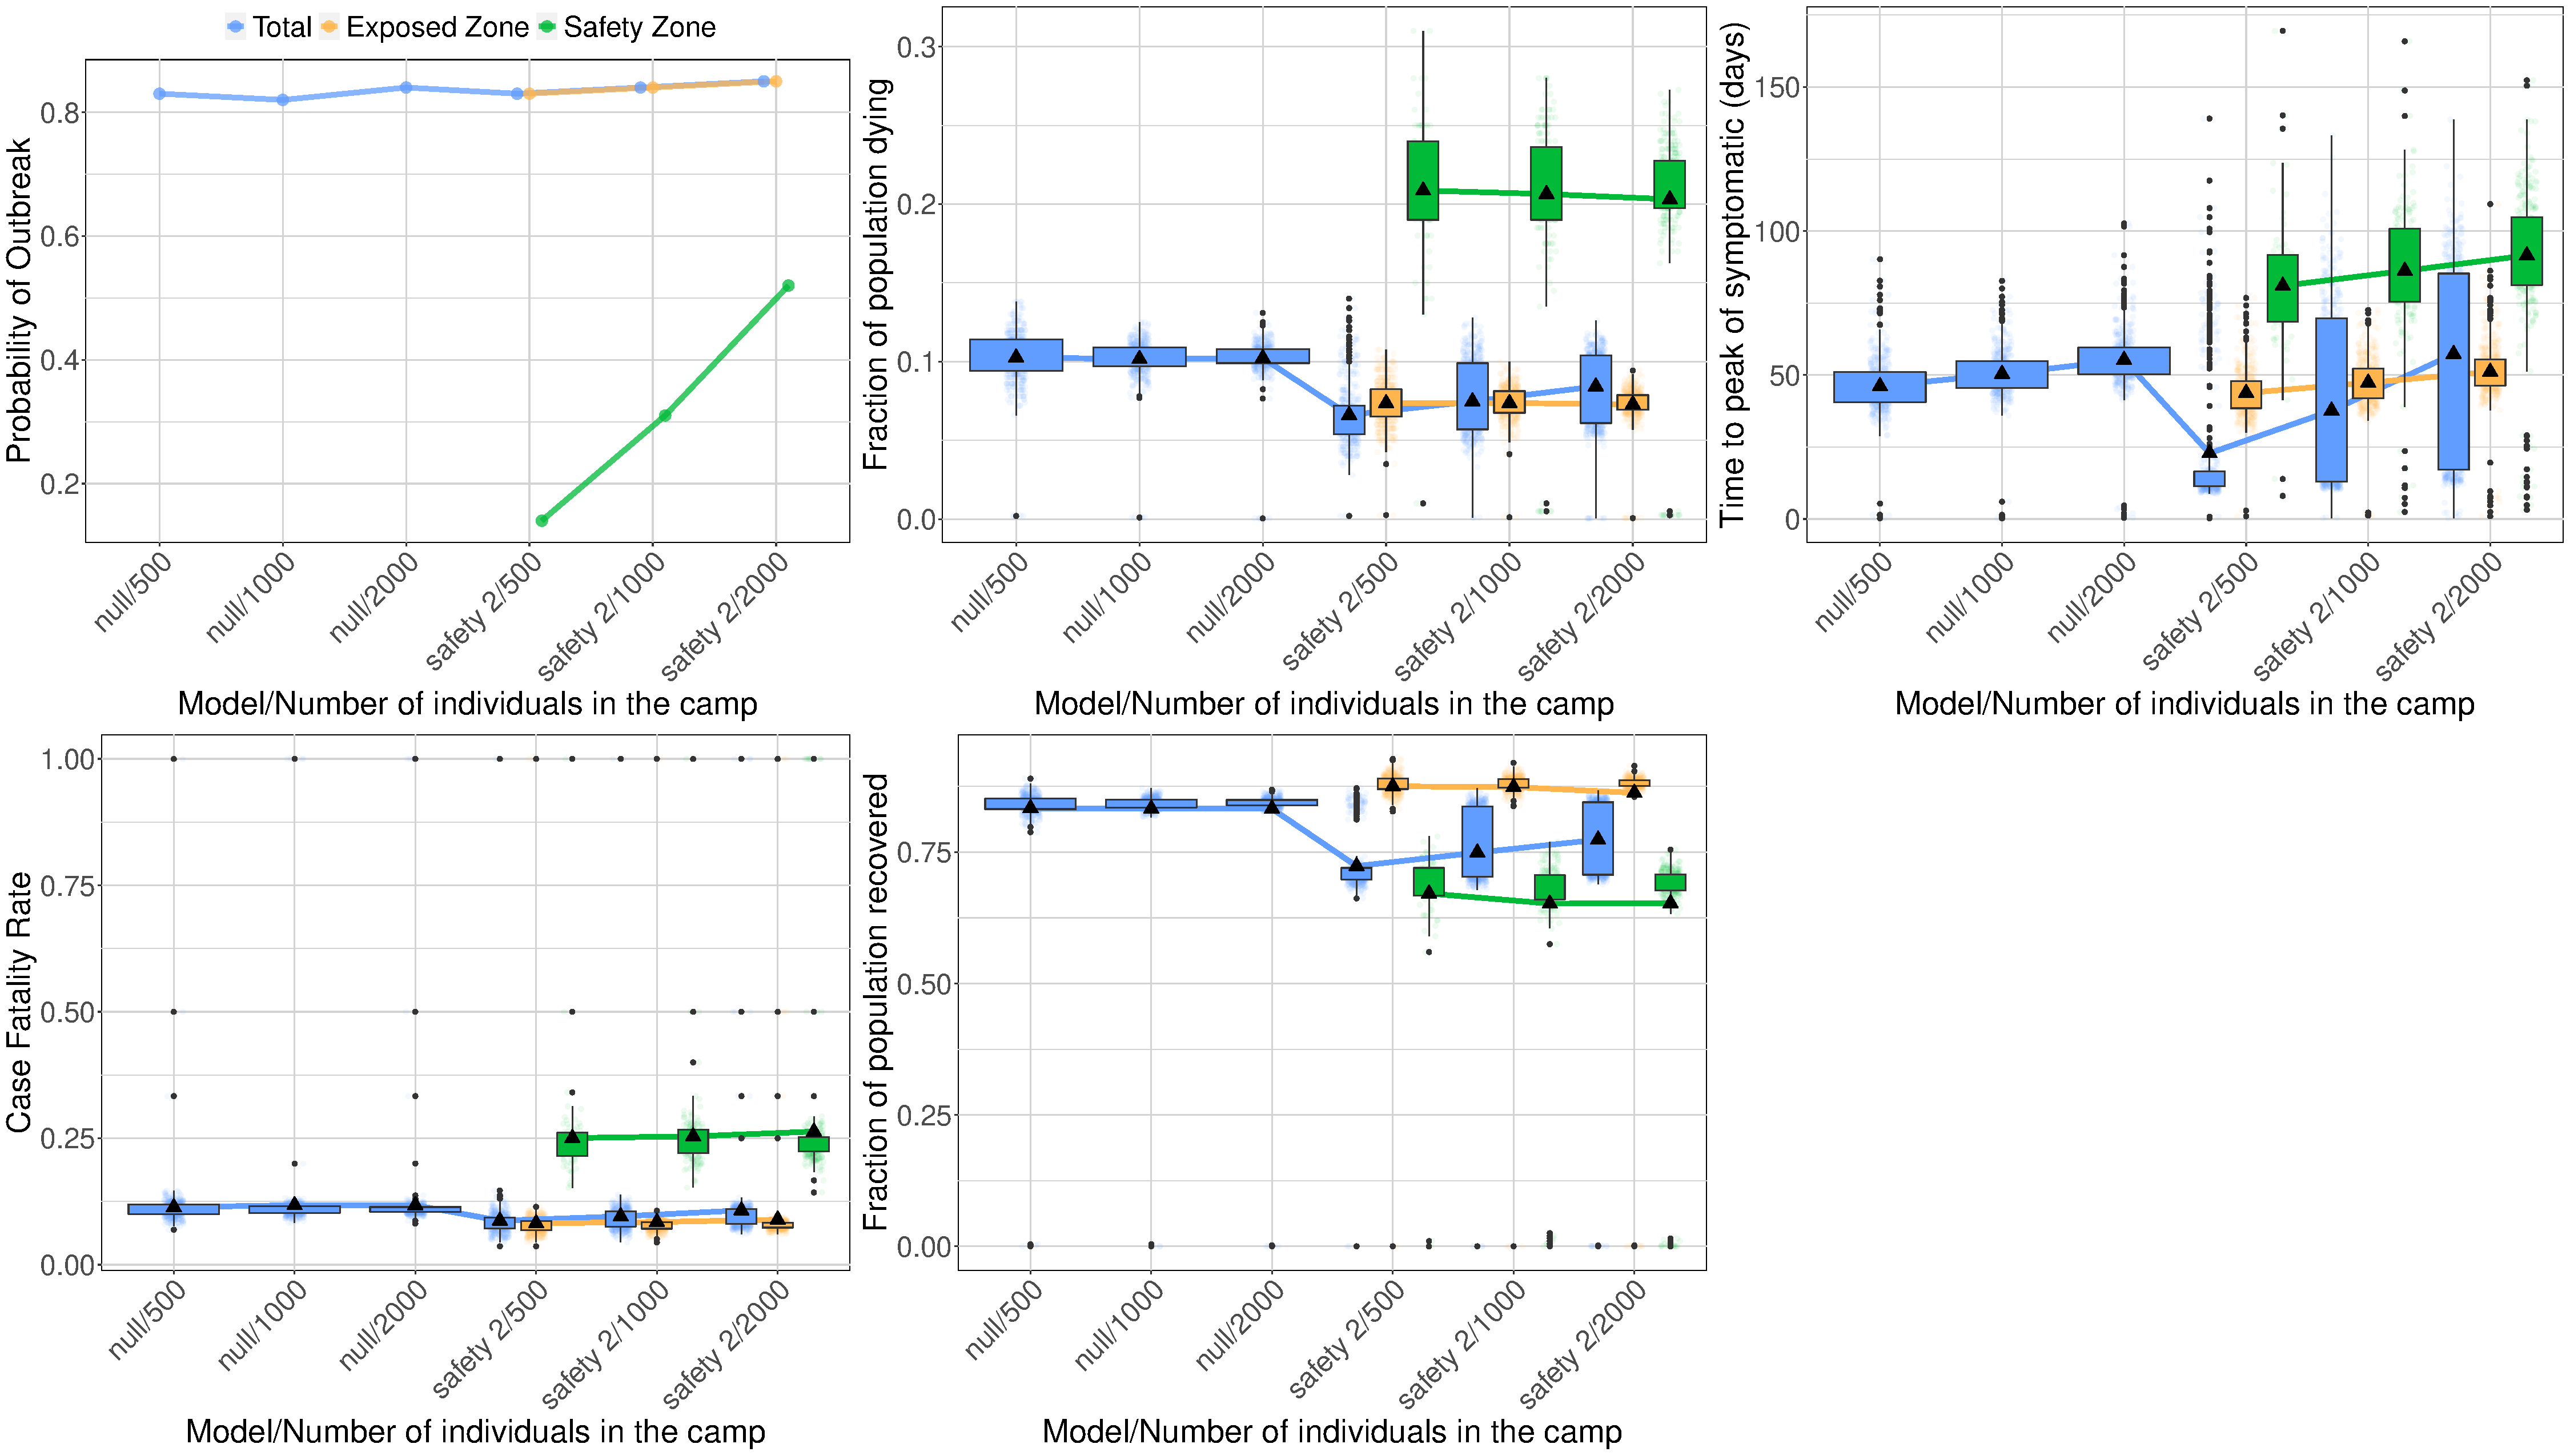
\includegraphics[width=1\textwidth]{figures/FigS10}\hspace{2mm}
\par\end{centering}
\caption{\label{fig:Suppl_popClass} \textbf{Population moving to the safety
zone.} Probability of an outbreak (top left), fraction of the population
dying (top middle), time until peak symptomatic cases (top right),
CFR (bottom left), and fraction of the population that recovers (bottom
middle) as a function of the safety zone allocation scenario (see
Table \ref{tab:SafetyScenarios}). All figures consider the scenario
with 2 contacts in the buffer per person in the safety zone per week.}
\end{figure}
\medskip{}

\begin{figure}[H]
\begin{centering}
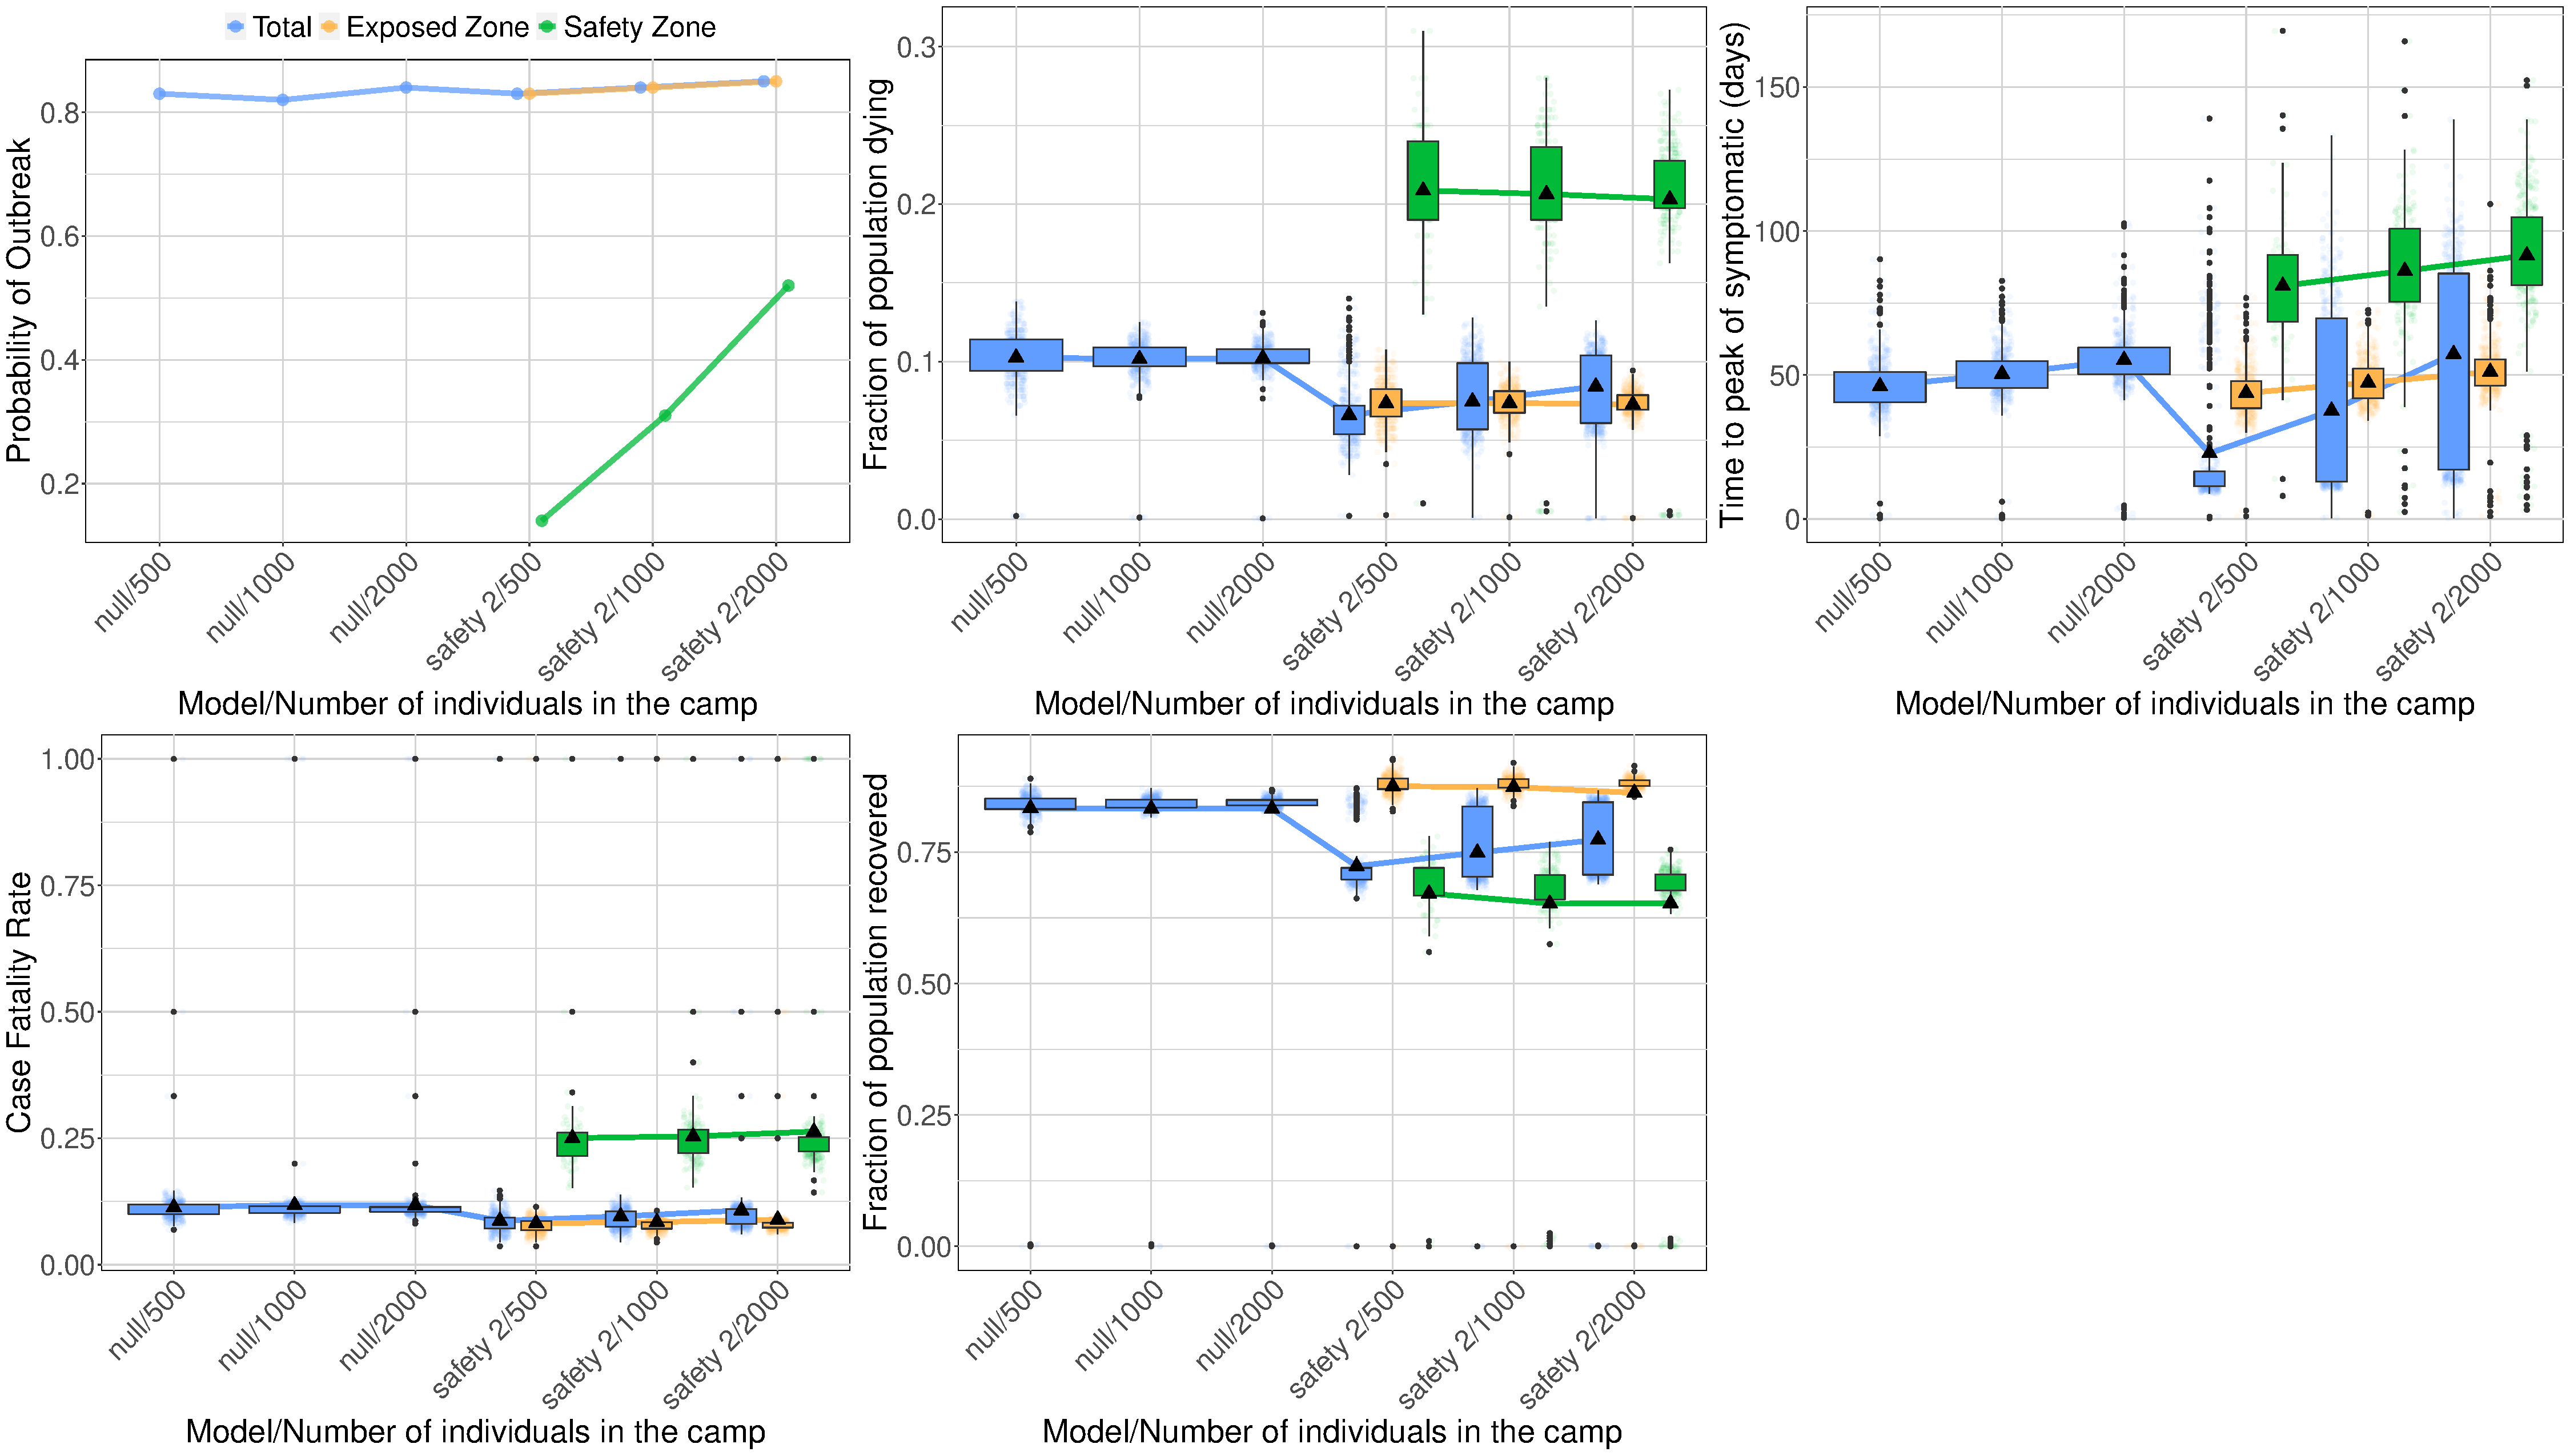
\includegraphics[width=1\textwidth]{figures/FigS11}\hspace{2mm}
\par\end{centering}
\caption{\label{fig:Suppl_popSize} \textbf{Efficacy of the safety zone for
different population sizes.} Probability of an outbreak (top left),
fraction of the population dying (top middle), time until peak symptomatic
cases (top right), CFR (bottom left), and fraction of the population
that recovers (bottom middle) as a function of the total population
size. The figures consider scenarios with no interventions (null),
and with a safety zone comprising 20\% of the camp's population with
2 contacts in the buffer zone per person in the safety zone per week
(safety 2).}
\end{figure}

\medskip{}

\begin{figure}[H]
\begin{centering}
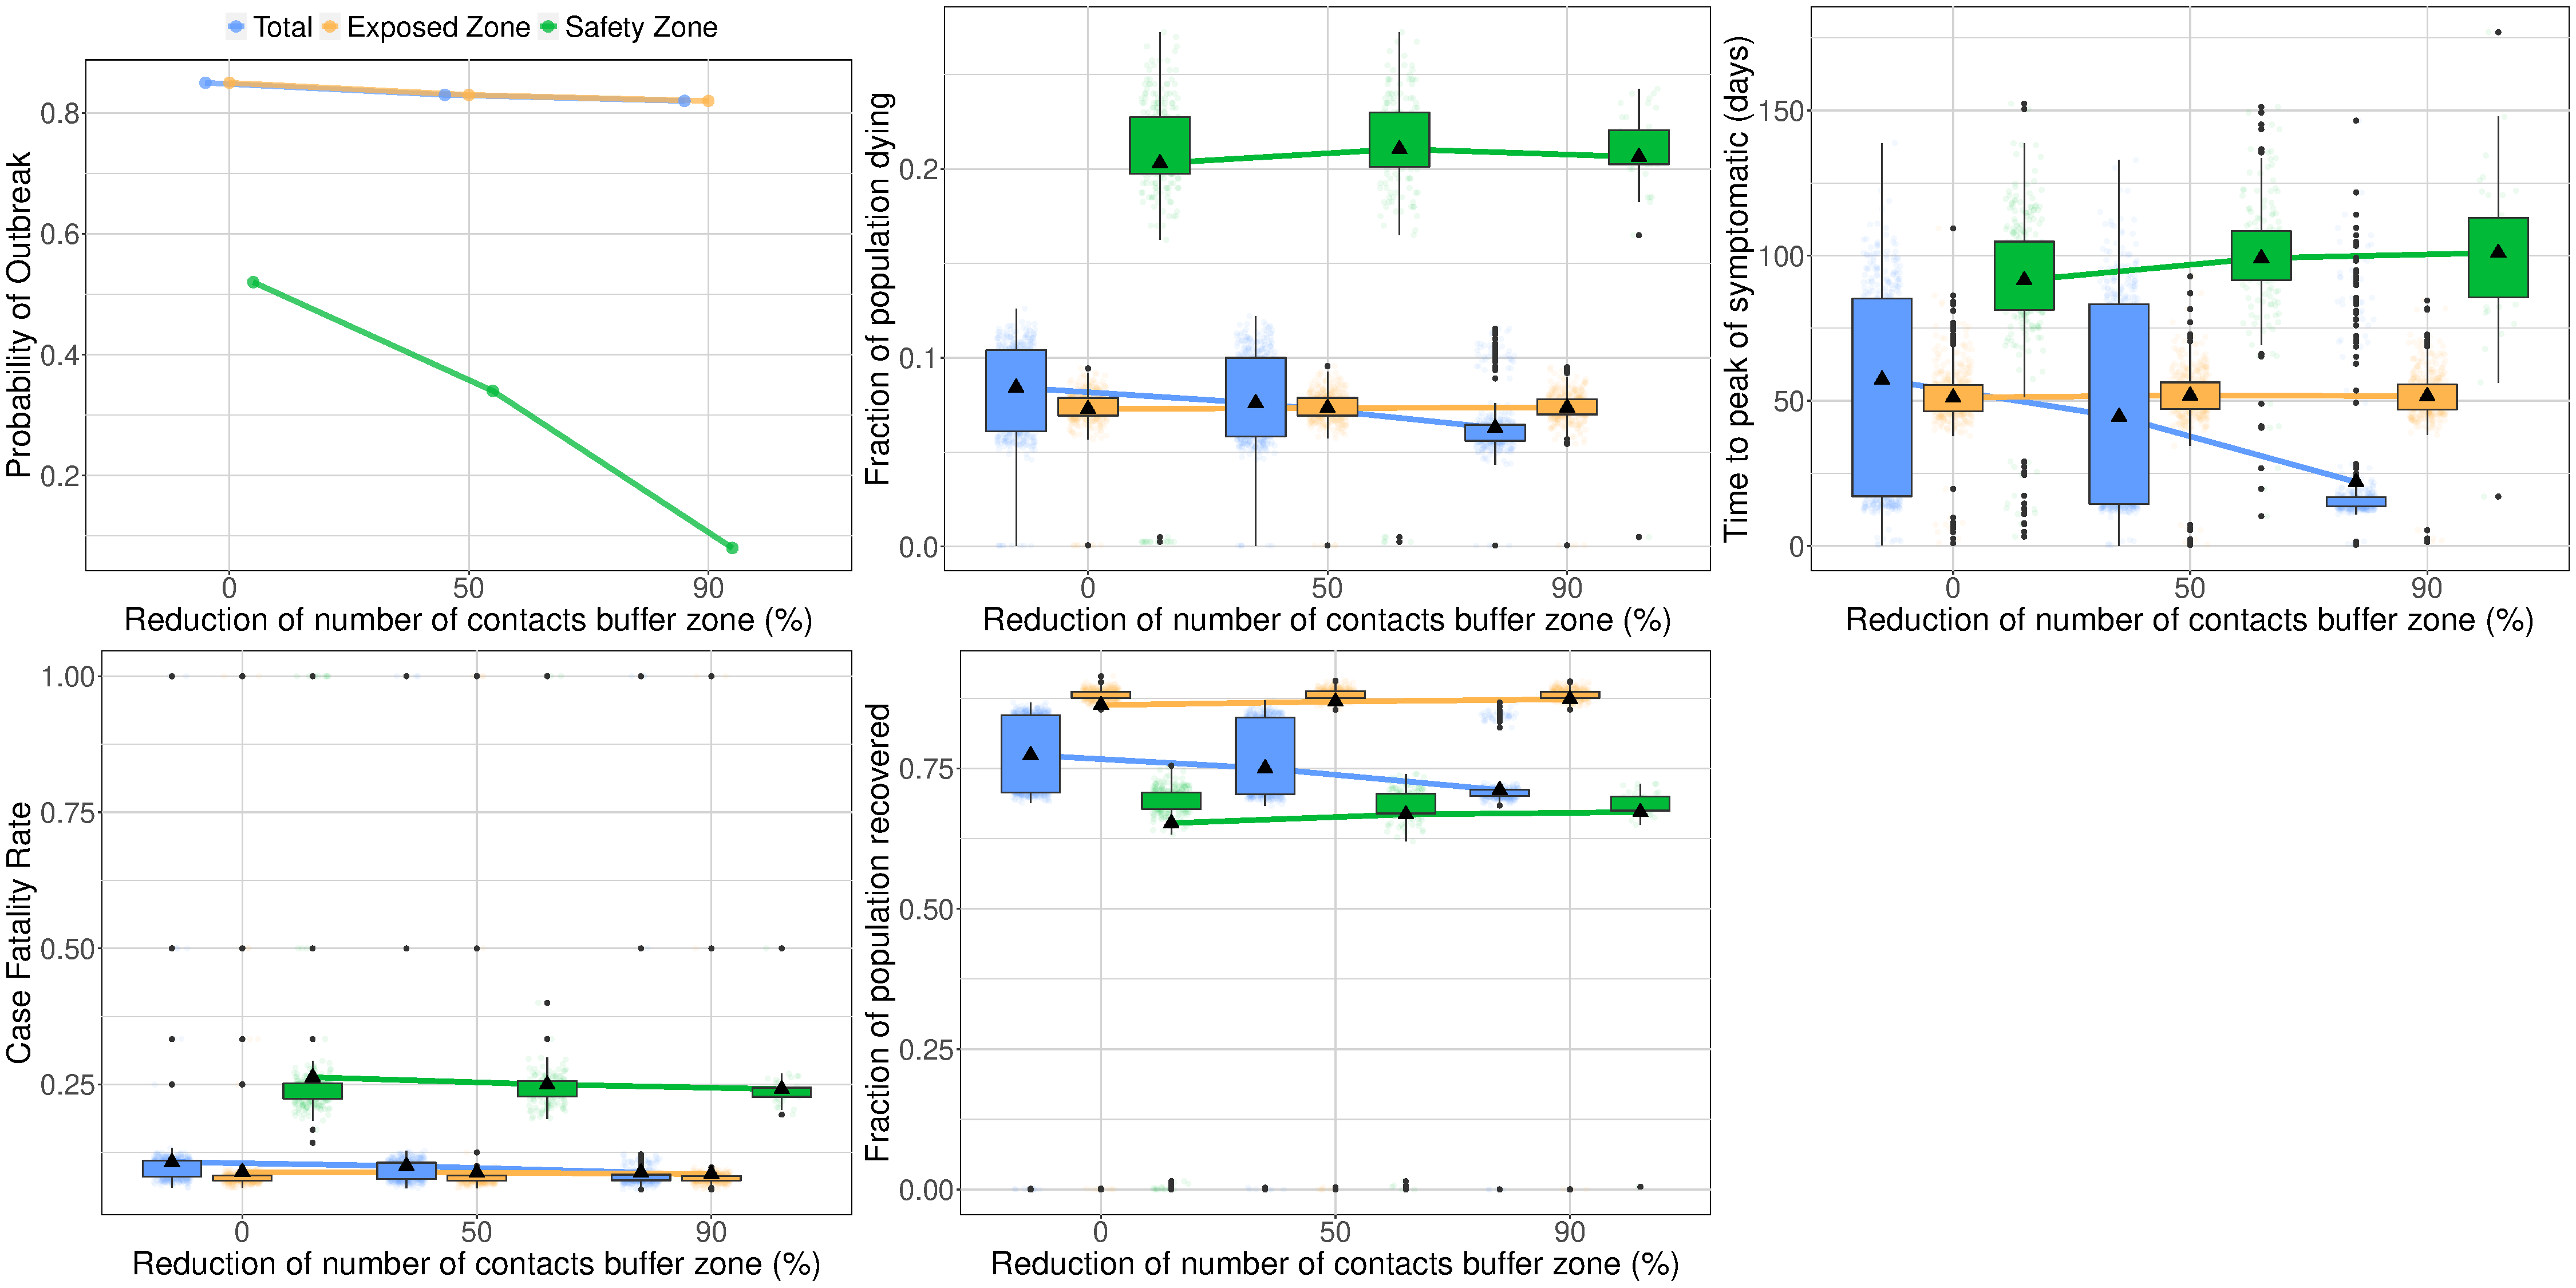
\includegraphics[width=1\textwidth]{figures/FigS12}\hspace{2mm}
\par\end{centering}
\caption{\label{fig:Suppl_lockdown} \textbf{Lockdown of the safety zone.}
Probability of an outbreak (top left), fraction of the population
dying (top middle), time until peak symptomatic cases (top right),
CFR (bottom left), and fraction of the population that recovers (bottom
middle) as a function of the reduction in the number of contacts permitted
in the buffer zone from a baseline of 2 per person in the safety zone
per week. All figures consider the scenario in which 20\% of the camp's
population is allocated to the safety zone.}
\end{figure}

\medskip{}

\begin{figure}[H]
\centering{}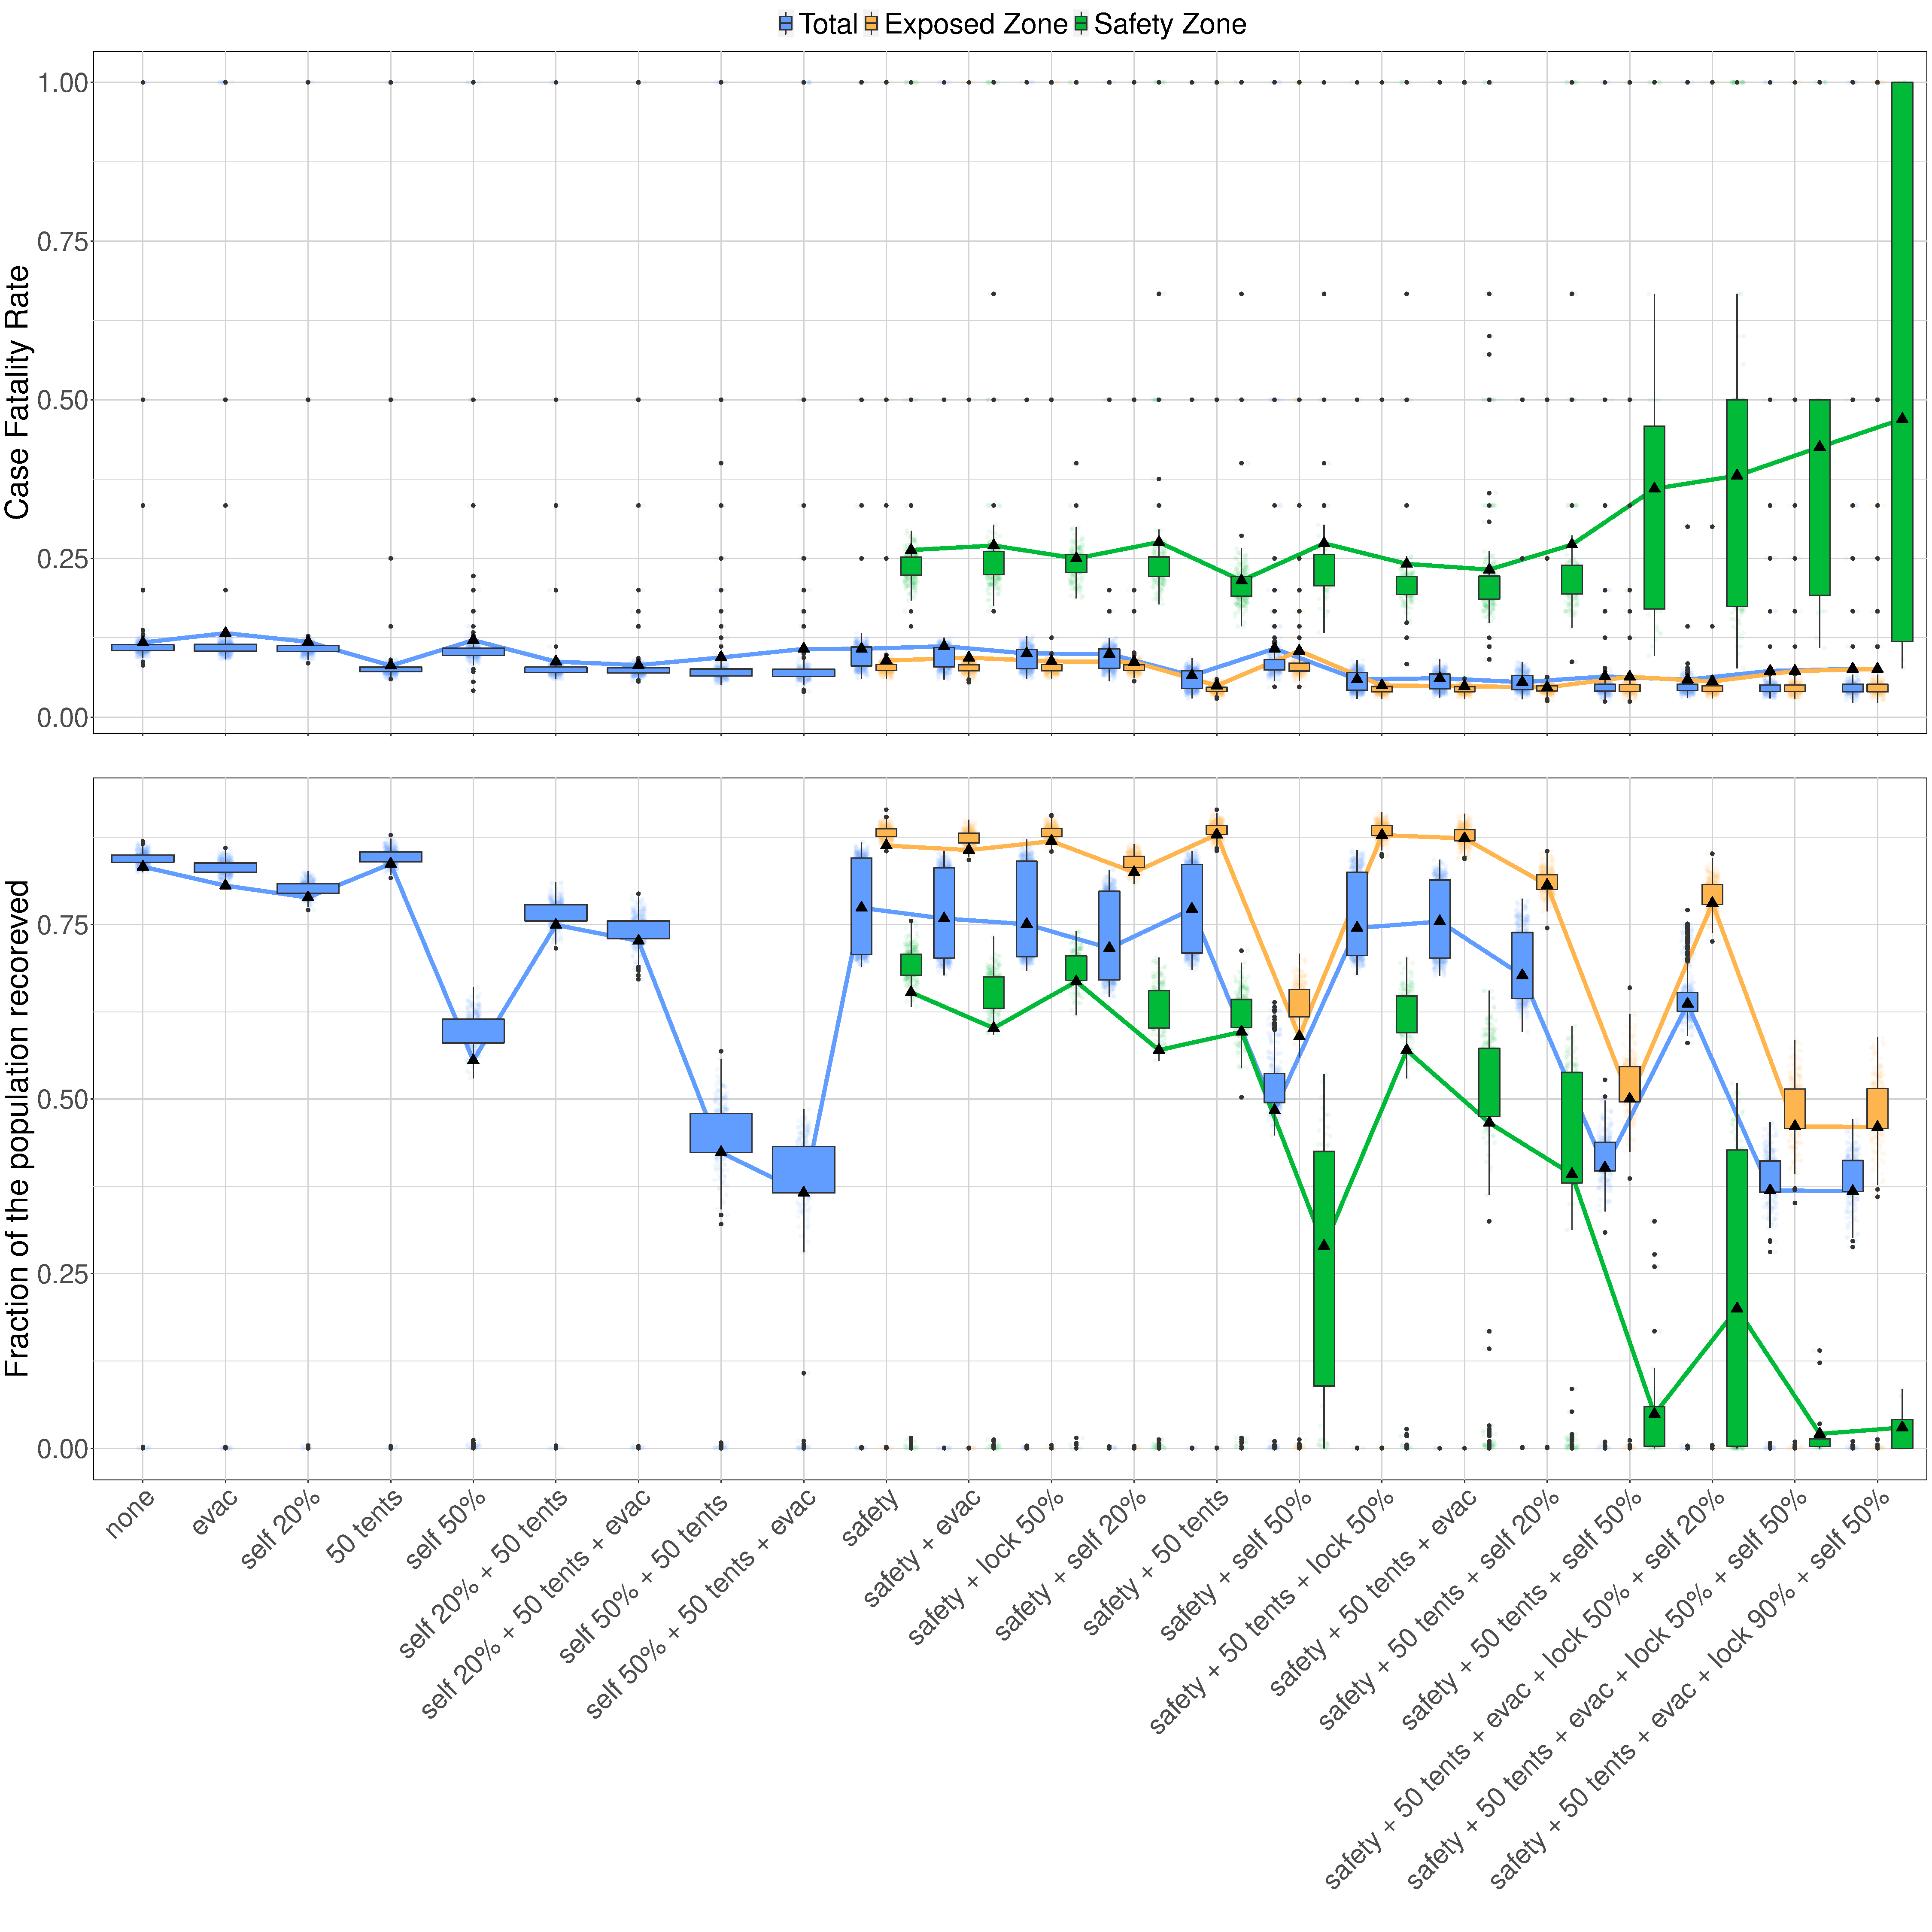
\includegraphics[width=1\textwidth]{figures/Fig_S13}\hspace{2mm}\caption{\label{fig:Suppl_combined} \textbf{Combined interventions.} CFR (top),
and fraction of the population that recovers (bottom) for different
combinations of interventions. Evac = evacuation of severely symptomatic,
self = self-distancing, tents = number of available self-isolation
tents, safety = safety zone, lock = lockdown of the buffer zone. For
combinations of interventions including a safety zone, we distinguish
between the population living in the green zone, in the orange zone
and the whole population. The increase in the CFR for the green zone
is explained by the discretization of the possible values that the
CFR can take when the number of cases is very low (see Supplementary
Table \ref{tab:CFR_discrete}).}
\end{figure}

\begin{table}[H]
\begin{centering}
\includegraphics{figures/Table_S4}
\par\end{centering}
\caption{\label{tab:CFR_discrete} \textbf{Efficacy of the safety zone in combination
with other interventions.} \textless 20 cases = number of outbreaks
in the green zone with fewer than 20 cases recorded. Total = total
number of simulations where an outbreak in the green zone occurs (at
least one death). \% of total = percent of outbreaks where fewer than
20 cases are recorded. N = 500 simulations for each combination of
interventions. For the most effective combinations, the majority of
simulations where an outbreak occurs in the green zone see fewer than
20 cases. In these simulations, the discretization of the possible
values that the CFR can take explains its apparently anomalous increase
in Fig. \ref{fig:Suppl_combined}.}
\end{table}

\newpage{}

\bibliographystyle{unsrt}
\bibliography{req550-syria}

\end{document}
